\documentclass[french]{beamer}
\usefonttheme[onlymath]{serif}
\usepackage[utf8]{inputenc}
\usepackage[T1]{fontenc}
\usepackage{lmodern}
\usepackage{babel}
\usepackage{tikz}
\usepackage{smartdiagram}
\usepackage{tabularx}
\usepackage[babel]{csquotes}
\usepackage[url=false, doi=false, style=science, backend=bibtex, bibencoding=ascii]{biblatex}
%\bibliography{IEEEabrv,bib/OAM}


\graphicspath{{img/}{../}}

\usepackage{../beamerthemeulaval}
\usepackage{../beamercolorthemeulaval}
\logo{\includegraphics[height=0.5cm]{UL_P}\hspace{.2cm}\vspace{.85\paperheight}}
\newcommand\red[1]{{\color{ulred}{\textbf{#1}}}}

\mode<presentation> {
	\setbeamercovered{invisible}
	\setbeamertemplate{navigation symbols}{} % Enlever les icônes de navigation
}

\title[Visualisation]{Visualiser des données}
%\subtitle[]{}

\author[C. Besse]{Camille Besse}
\institute[Université Laval]
{
	Départment d'Informatique et de Génie Logiciel\\
	Université Laval, Québec, Canada \\
	\medskip
	{\emph{camille.besse@ift.ulaval.ca}}
}
%\date{\today} % \today will show current date. 
% Alternatively, you can specify a date.


\AtBeginSection[]{
 \begin{frame}
	\Huge \centerline{\insertsection}
%  \small \tableofcontents[currentsection, hideothersubsections]
  \end{frame} 
}

\begin{document}



%---------------------------------------------------------------------------------------------------------------------------------------- 
 \begin{frame}[label=titre, plain]
	\titlepage
	\begin{center}\includegraphics[height=1cm]{UL_P}\end{center}
\end{frame}


%---------------------------------------------------------------------------------------------------------------------------------------- 
 \begin{frame}[label=src]{Source}
\begin{center}
Présentation originale de John Rauser

{\Huge "How Humans See Data"}

\vspace{1cm}
{\footnotesize Si vous préférez écouter la version originale

Original material in R : \\
\url{https://github.com/jrauser/writing/blob/master/how_humans_see_data/}}

\vspace{1cm}
{\tiny Complété un peu avec de trucs de \url{http://www.perceptualedge.com}
	
et de \url{http://ieg.ifs.tuwien.ac.at/~aigner/}}

\end{center}

\end{frame}



\section*{Contents}

%---------------------------------------------------------------------------------------------------------------------------------------- 
 \begin{frame}[label=toc]{Outline}

	\begin{itemize}
		\item Pourquoi visualiser des données ?
		\item Perception et schémas
		\begin{itemize}
			\item Détection
			\item Montage
			\item 	Estimation
		\end{itemize}
		\item Quelques autres trucs…
	\end{itemize}

\end{frame}

%---------------------------------------------------------------------------------------------------------------------------------------- 
 \begin{frame}{Visualisation}
\begin{itemize}
	\item Pourquoi visualiser ?
	\item La visualisation est de la communication
	\item Le but est de permettre à des humains de résoudre un problème analytique rapidement et précisément
\end{itemize}
\end{frame}

%---------------------------------------------------------------------------------------------------------------------------------------- 
 \begin{frame}{Visualisation}
\begin{itemize}
	\item Pourquoi visualiser ?
	\item La visualisation est de la communication
	\item Le but est de permettre à des humains de résoudre un problème analytique rapidement et précisément
\end{itemize}
\end{frame}

%---------------------------------------------------------------------------------------------------------------------------------------- 
 \begin{frame}{Des données ... }
	\vspace{-0.2cm}
	\hspace*{-0.9cm}
	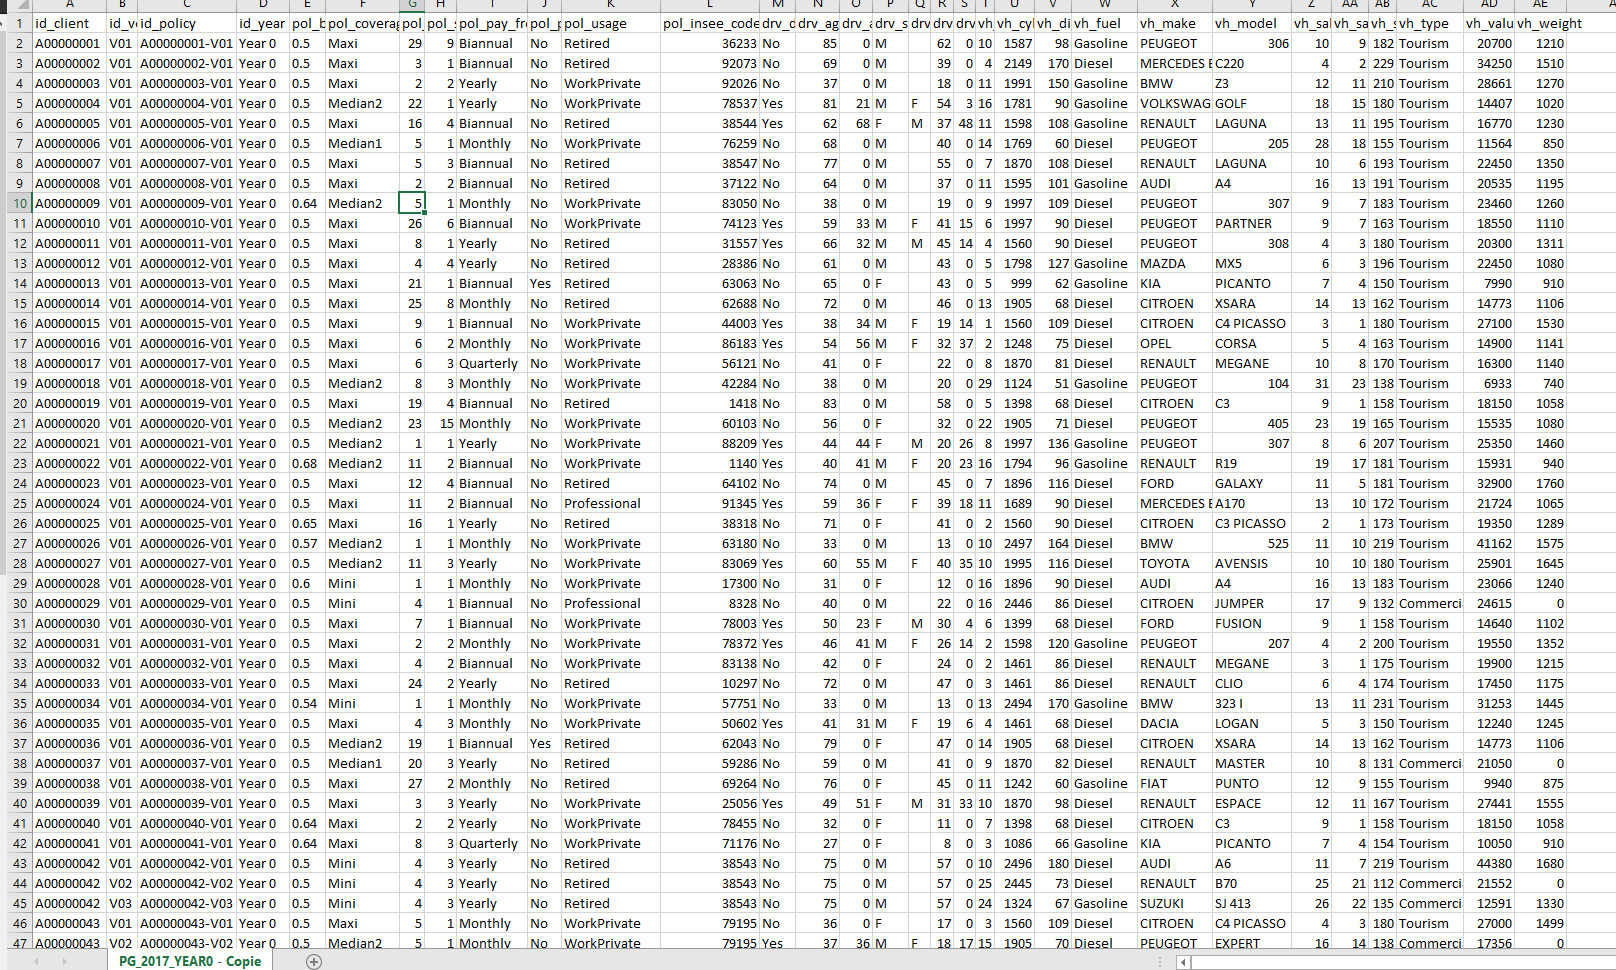
\includegraphics[width=1.2\textwidth]{data}
\end{frame}

%---------------------------------------------------------------------------------------------------------------------------------------- 
 \begin{frame}{... brutes.}
\begin{center}
	\begin{tabular}{|cc|c|cc|}
		x & y  &  & x & y \\ 
		1.972&1.236&&0.111&0.542 \\
		1.112&1.994&&0.902&0.005 \\
		0.000&1.009&&0.598&0.085 \\
		0.665&1.942&&1.613&1.790 \\
		0.235&0.356&&1.298&1.955 \\
		0.247&1.658&&0.651&1.937 \\
		1.275&1.961&&1.949&1.316 \\
		0.702&0.045&&0.099&0.567 \\
		1.760&0.350&&0.862&0.010 \\
		1.691&0.277&&0.027&0.768 \\
		1.628&1.778&&0.706&1.956 \\
		1.957&1.290&&1.042&1.999 \\
	\end{tabular} 
\end{center}
\end{frame}

%---------------------------------------------------------------------------------------------------------------------------------------- 
 \begin{frame}{justes brutes .... mais ... }
\begin{minipage}{.49\textwidth}
\begin{center}
	\begin{tabular}{|cc|c|cc|}
		x & y  &  & x & y \\ 
		1.972&1.236&&0.111&0.542 \\
		1.112&1.994&&0.902&0.005 \\
		0.000&1.009&&0.598&0.085 \\
		0.665&1.942&&1.613&1.790 \\
		0.235&0.356&&1.298&1.955 \\
		0.247&1.658&&0.651&1.937 \\
		1.275&1.961&&1.949&1.316 \\
		0.702&0.045&&0.099&0.567 \\
		1.760&0.350&&0.862&0.010 \\
		1.691&0.277&&0.027&0.768 \\
		1.628&1.778&&0.706&1.956 \\
		1.957&1.290&&1.042&1.999 \\
	\end{tabular} 
\end{center}
\end{minipage}\hfill
\begin{minipage}{.45\textwidth}
	\begin{center}
	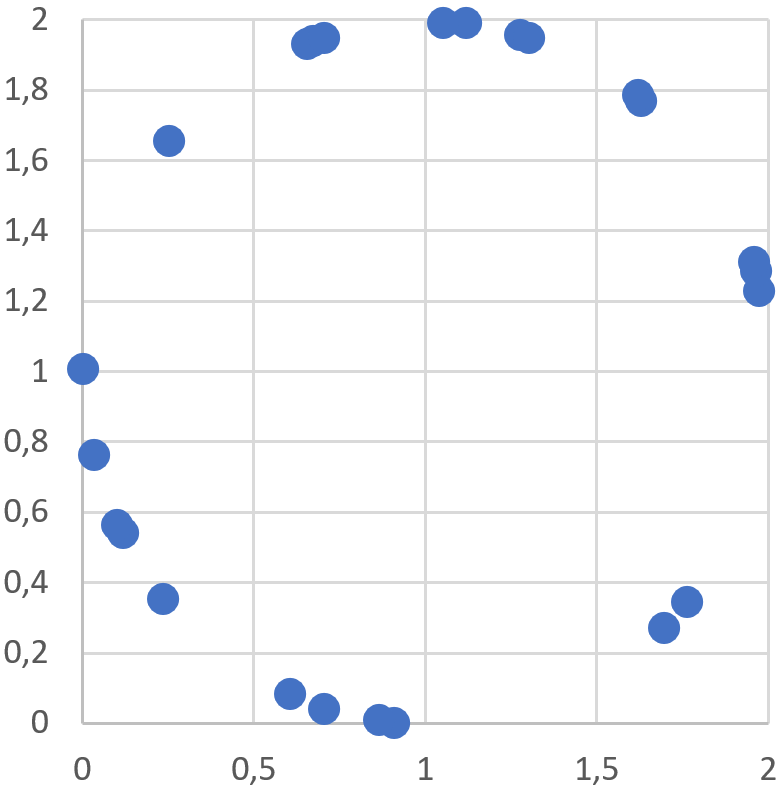
\includegraphics[width=\textwidth]{circle}
	\end{center}
\end{minipage}
\end{frame}

%---------------------------------------------------------------------------------------------------------------------------------------- 
 \begin{frame}{}
\begin{center}\begin{Huge}\textbf{
	Un graphique est un\\ \red{encodage}\\ de données.
}\end{Huge}\end{center}
\end{frame}

%---------------------------------------------------------------------------------------------------------------------------------------- 
 \begin{frame}{Et si ...}
\begin{center}
	\begin{tabular}{r|cc|cr|cc|}
		n&x & y  &  & n& x & y \\ 
		1&1.972&1.236&& 13&0.111&0.542 \\
		2&1.112&1.994&& 14&0.902&0.005 \\
		3&0.000&1.009&& 15&0.598&0.085 \\
		4&0.665&1.942&& 16&1.613&1.790 \\
		5&0.235&0.356&& 17&1.298&1.955 \\
		6&0.247&1.658&& 18&0.651&1.937 \\
		7&1.275&1.961&& 19&1.949&1.316 \\
		8&0.702&0.045&& 20&0.099&0.567 \\
		9&1.760&0.350&& 21&0.862&0.010 \\
		10&1.691&0.277&& 22&0.027&0.768 \\
		11&1.628&1.778&& 23&0.706&1.956 \\
		12&1.957&1.290&& 24&1.042&1.999 \\
	\end{tabular} 
\end{center}
\end{frame}

%---------------------------------------------------------------------------------------------------------------------------------------- 
 \begin{frame}{... on fait pas attention ...}
\begin{minipage}{.49\textwidth}
	\begin{center}
	\resizebox{\textwidth}{!}{
		\begin{tabular}{r|cc|cr|cc|}
		n&x & y  &  & n& x & y \\ 
		1&1.972&1.236&& 13&0.111&0.542 \\
		2&1.112&1.994&& 14&0.902&0.005 \\
		3&0.000&1.009&& 15&0.598&0.085 \\
		4&0.665&1.942&& 16&1.613&1.790 \\
		5&0.235&0.356&& 17&1.298&1.955 \\
		6&0.247&1.658&& 18&0.651&1.937 \\
		7&1.275&1.961&& 19&1.949&1.316 \\
		8&0.702&0.045&& 20&0.099&0.567 \\
		9&1.760&0.350&& 21&0.862&0.010 \\
		10&1.691&0.277&& 22&0.027&0.768 \\
		11&1.628&1.778&& 23&0.706&1.956 \\
		12&1.957&1.290&& 24&1.042&1.999 \\
		\end{tabular} }
	\end{center}
\end{minipage}
\hfill
\begin{minipage}{.45\textwidth}
	\begin{center}
		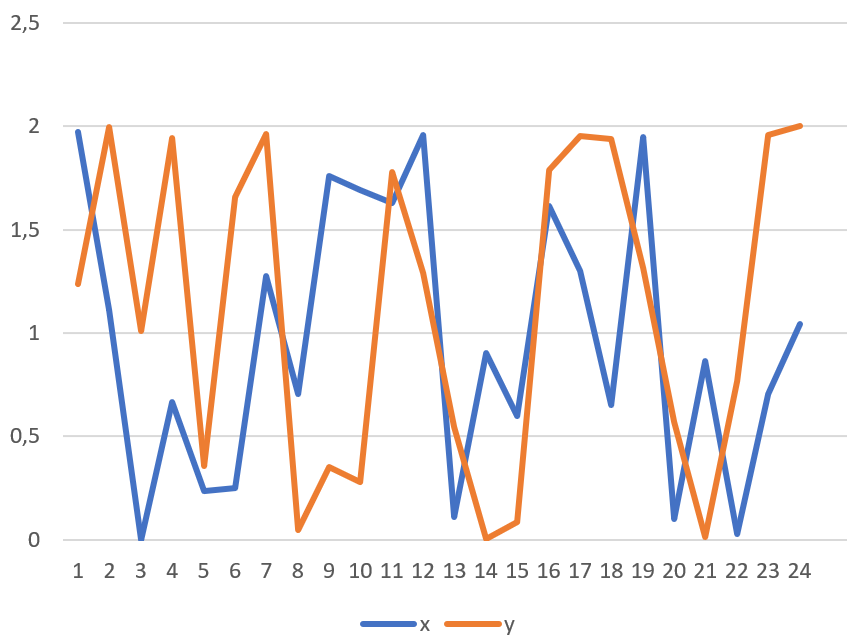
\includegraphics[width=\textwidth]{line}
	\end{center}
\end{minipage}
\end{frame}

%---------------------------------------------------------------------------------------------------------------------------------------- 
 \begin{frame}{}
\begin{center}\begin{Huge}\textbf{
			Les bons visuels \red{optimisent}\\
			le système cognitif \red{humain.}
}\end{Huge}\end{center}
\end{frame}

%---------------------------------------------------------------------------------------------------------------------------------------- 
 \begin{frame}{LE livre}
\begin{minipage}{.49\textwidth}{\LARGE 
Mais comment l'être humain décode t'il un graphique ?
}\end{minipage}
\hfill
\begin{minipage}{.49\textwidth}
	\begin{center}
		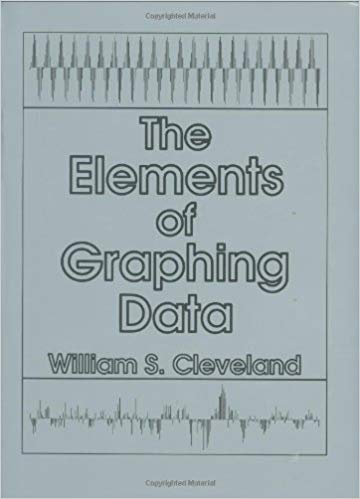
\includegraphics[width=\textwidth]{book}
	\end{center}
\end{minipage}
\end{frame}

%---------------------------------------------------------------------------------------------------------------------------------------- 
 \begin{frame}{Outline}
Trois opérations visuelles dans la perception de shémas : 
\begin{enumerate}
	\item Détection
	\item Construction
	\item Estimation
\end{enumerate}
\end{frame}

\section{Estimation}

%---------------------------------------------------------------------------------------------------------------------------------------- 
 \begin{frame}{Estimation}
Trois niveau d'estimation : 
\begin{enumerate}
	\item Discrimination \hfill $X = Y$ ou $X \neq Y$ ?
	\item Ordre \hfill $X < Y$ ou $X > Y$ ?
	\item Ratio\hfill $X / Y = $ ?
\end{enumerate}
\end{frame}

%---------------------------------------------------------------------------------------------------------------------------------------- 
\begin{frame}{}
\begin{large}
		"Au coeur du raisonnement quantitatif existe une seule question : \\
		Comparé à quoi ?"
		
\vspace{1cm}
\textit{- Tufte, Envisioning Information}
\end{large}
\end{frame}

%---------------------------------------------------------------------------------------------------------------------------------------- 
 \begin{frame}{En 1985}
\begin{large}
\textbf{Graphical Perception and Graphical Methods for Analyzing Scientific Data}

\vspace{0.7cm}
\textit{William S. Cleveland and Robert McGill}

\vspace{1cm}
Science 30 Aug 1985\\
Vol. 229, Issue 4716, pp. 828-833\\
DOI: 10.1126/science.229.4716.828
\end{large}
\end{frame}

%---------------------------------------------------------------------------------------------------------------------------------------- 
\begin{frame}{En 1985}
	\begin{center}
	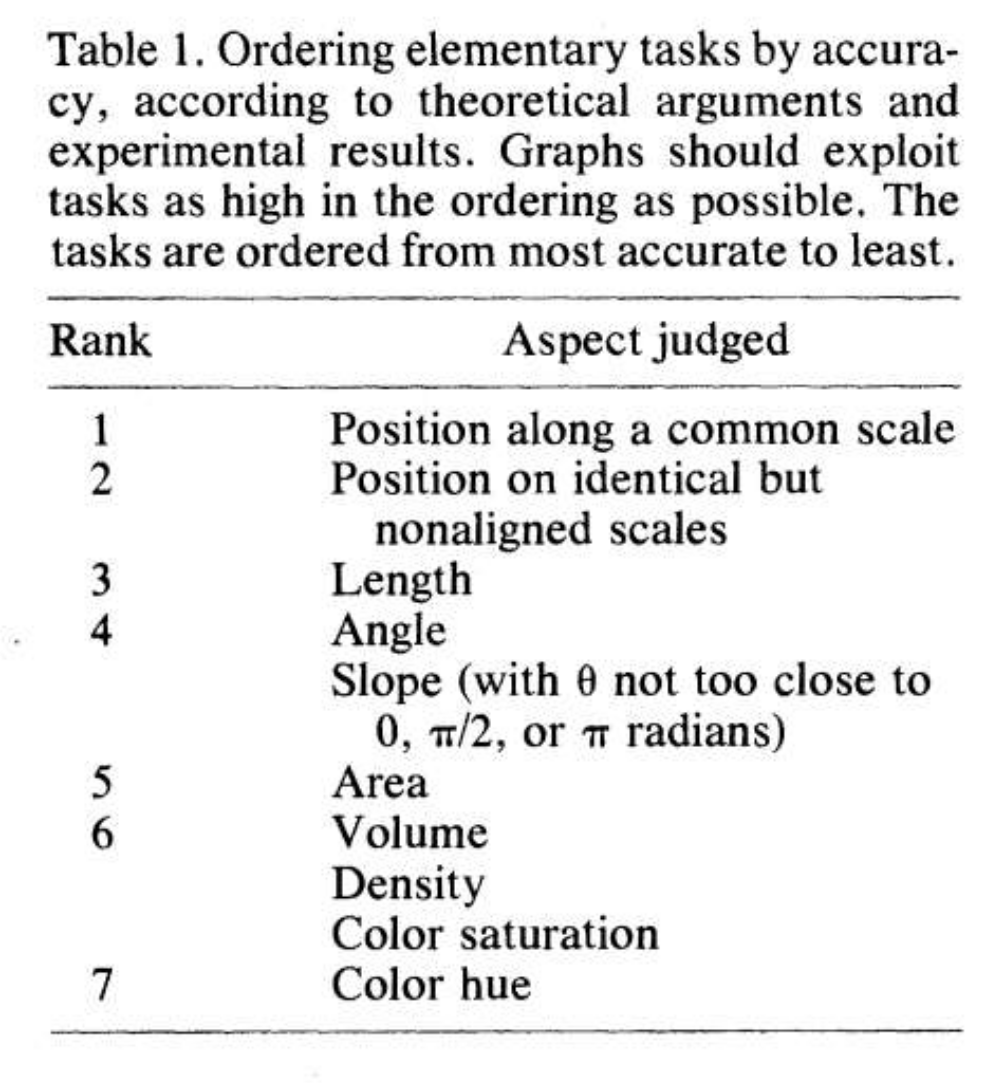
\includegraphics[height=0.8\textheight]{liste}
\end{center}
\end{frame}

%---------------------------------------------------------------------------------------------------------------------------------------- 
 \begin{frame}{}
\begin{center}\begin{Huge}\textbf{
			La chose la plus\\
			\red{importante}
}\end{Huge}\end{center}
\end{frame}

%---------------------------------------------------------------------------------------------------------------------------------------- 
\begin{frame}{En 1985}
\begin{center}
	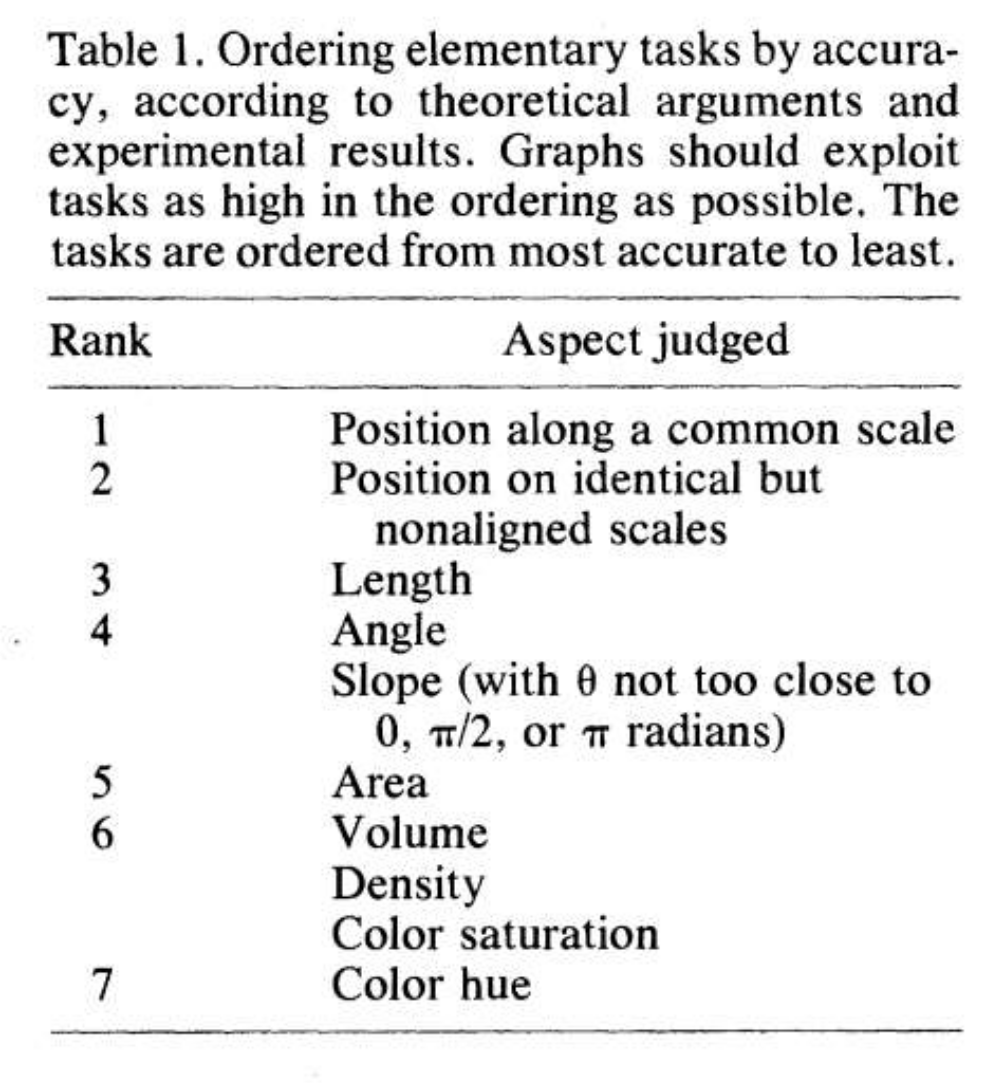
\includegraphics[height=0.8\textheight]{liste}
\end{center}
\end{frame}

%---------------------------------------------------------------------------------------------------------------------------------------- 
 \begin{frame}{Ordre d'encodage}
La mesure la plus importante devrait exploiter l'encodage ayant le rang le plus haut :
\begin{enumerate}
	\item Position sur une échelle commune
	\item Position sur une échelle identique non alignée
	\item Longueur
	\item Angle ou pente
	\item Aire
	\item Volume ou Densité ou Saturation de couleur
	\only<1>{\item Teinte de couleur}
	\only<2>{\item \red{Teinte de couleur}}
\end{enumerate}
\end{frame}

%---------------------------------------------------------------------------------------------------------------------------------------- 
\begin{frame}{}
\begin{Large}
	“Première règle de la couleur : \\
	On ne parle pas de la couleur !”

	\vspace{1cm}
	\textit{- Tamara Munzner}
\end{Large}
\end{frame}

%---------------------------------------------------------------------------------------------------------------------------------------- 
\newcommand\img[1]{\raisebox{-0.5\height}{\includegraphics[height=2cm]{#1}}}
\begin{frame}{Couleur : 3 composantes}
	\begin{tabularx}{\textwidth}{Xr} 
		\renewcommand{\arraystretch}{2cm}
		Luminosité  & \img{grey}\\ 
		Saturation  & \img{saturation}\\ 
		Teinte 		& \img{hue}
	\end{tabularx} 
\end{frame}


%---------------------------------------------------------------------------------------------------------------------------------------- 
\newcommand\lb[1]{\color[HSB]{155,134,180}{#1}}
\newcommand\rb[1]{{\color[HSB]{155,134,100}{#1}}}
\begin{frame}{Exemple de saturation : Nombres}
\begin{center}
	\lb{\Large\textbf{
			1561321203658413076510374627\\
			4173127527327592732990709742\\
			1703707774179527931749270973\\
			4019743217909370945179279417\\
	}}
	
	\vspace{1cm}
	\lb{\Large\textbf{
			1\rb{5}613212036\rb{5}8413076\rb{5}10374627\\
			4173127\rb{5}27327\rb{5}92732990709742\\
			1703707774179\rb{5}27931749270973\\
			401974321790937094\rb{5}179279417\\
	}}
	
\end{center}
\end{frame}

%---------------------------------------------------------------------------------------------------------------------------------------- 
\begin{frame}{Exemple de Luminosité et teintes : scatter}
\begin{minipage}{.45\textwidth}
	\begin{center}
		Luminosité
		
		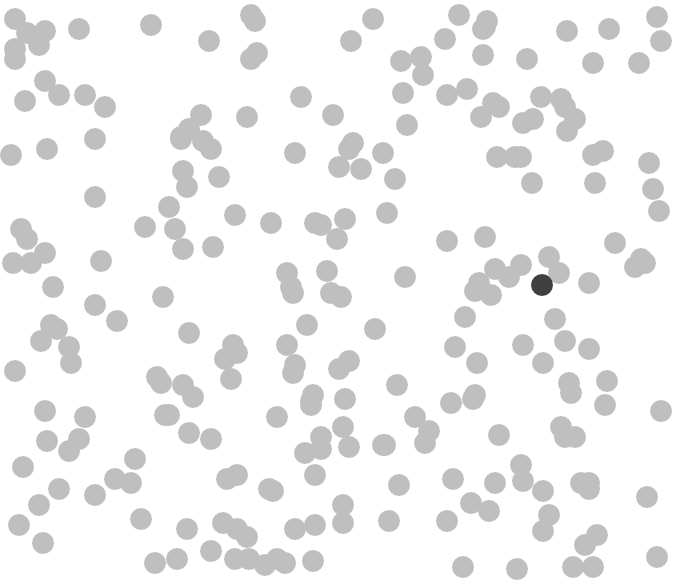
\includegraphics[width=\textwidth]{plotgrey}
	\end{center}
\end{minipage}
\hfill
\begin{minipage}{.45\textwidth}
	\begin{center}
		Teinte
		
		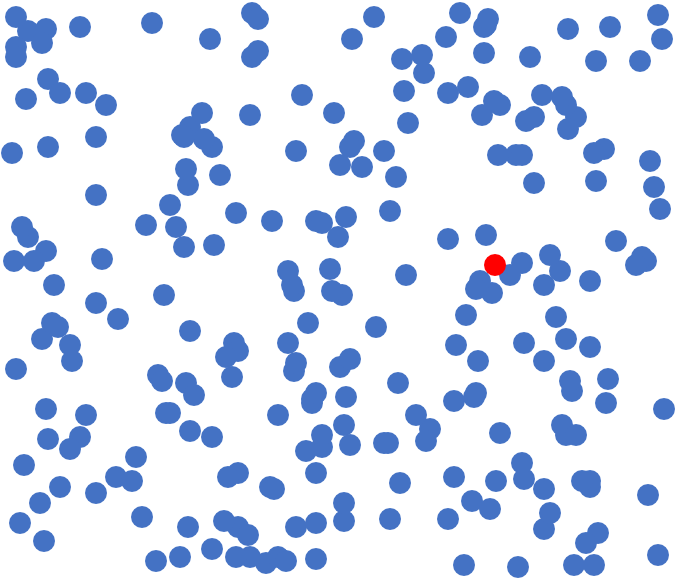
\includegraphics[width=\textwidth]{plothue}
	\end{center}
\end{minipage}
\end{frame}

%---------------------------------------------------------------------------------------------------------------------------------------- 
\begin{frame}{Exemple de teintes : dataset autos}
\begin{center}
	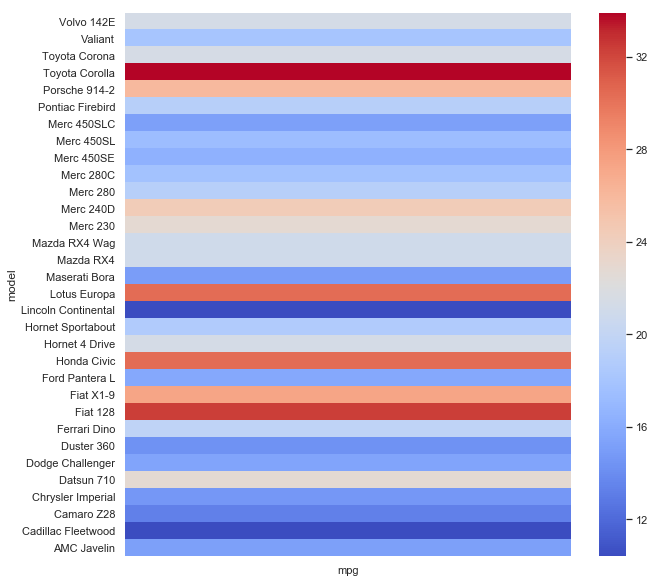
\includegraphics[height=0.8\textheight]{autoshue}
\end{center}
\end{frame}


%---------------------------------------------------------------------------------------------------------------------------------------- 
\begin{frame}{}
\begin{center}\begin{Huge}\textbf{
			L'ordre \red{alphabétique} est quasiment \red{jamais} le bon ordre pour une variable \red{catégorique}.
}\end{Huge}\end{center}
\end{frame}

%---------------------------------------------------------------------------------------------------------------------------------------- 
\begin{frame}{Exemple de teintes ordonnées : dataset autos}
\begin{center}
	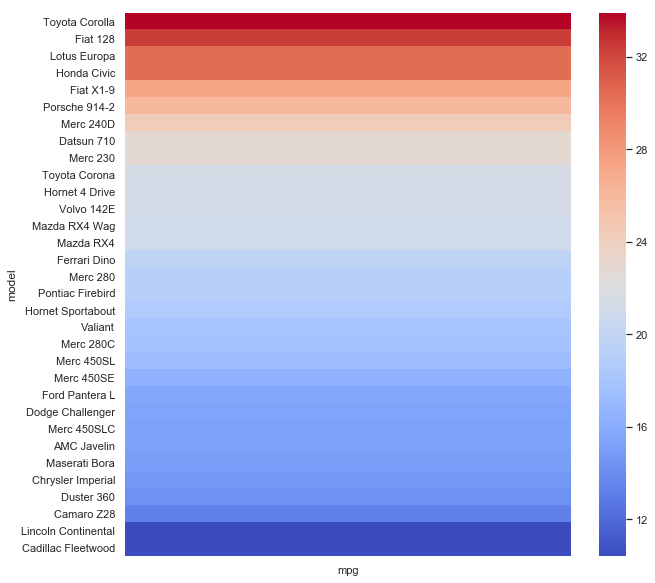
\includegraphics[height=0.8\textheight]{autoshue_order}
\end{center}
\end{frame}

%---------------------------------------------------------------------------------------------------------------------------------------- 
\begin{frame}{Ordre d'encodage}
La mesure la plus importante devrait exploiter l'encodage ayant le rang le plus haut :
\begin{enumerate}
	\item Position sur une échelle commune
	\item Position sur une échelle identique non alignée
	\item Longueur
	\item Angle ou pente
	\item Aire
	\item Volume ou Densité ou \red{Saturation de couleur}
	\item Teinte de couleur
\end{enumerate}
\end{frame}

%---------------------------------------------------------------------------------------------------------------------------------------- 
\begin{frame}{Exemple de saturations ordonnées : dataset autos}
\begin{center}
	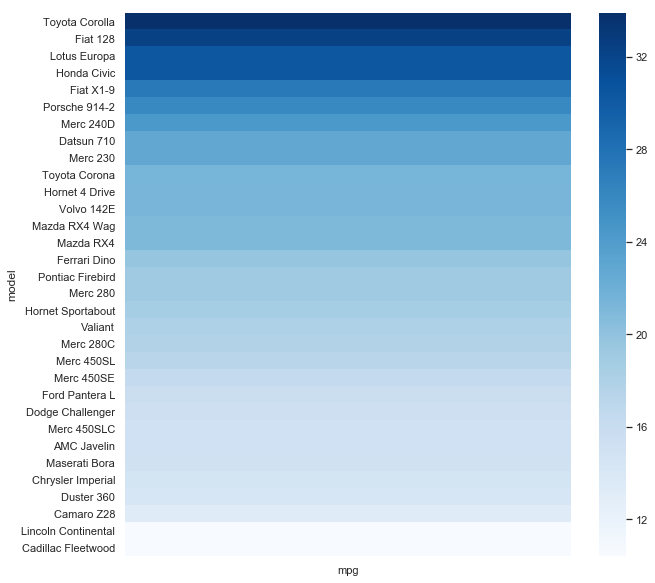
\includegraphics[height=0.8\textheight]{autossat_order}
\end{center}
\end{frame}

%---------------------------------------------------------------------------------------------------------------------------------------- 
\begin{frame}{Exemple de teintes ordonnées : dataset autos}
\begin{center}
	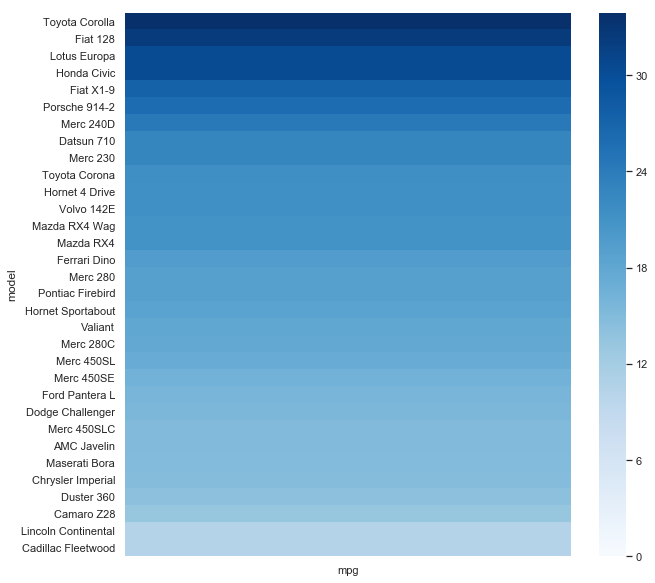
\includegraphics[height=0.8\textheight]{autossat_zero}
\end{center}
\end{frame}

%---------------------------------------------------------------------------------------------------------------------------------------- 
\begin{frame}{Ordre d'encodage}
La mesure la plus importante devrait exploiter l'encodage ayant le rang le plus haut :
\begin{enumerate}
	\item Position sur une échelle commune
	\item Position sur une échelle identique non alignée
	\item Longueur
	\item Angle ou pente
	\item \red{Aire}
	\item Volume ou Densité ou Saturation de couleur
	\item Teinte de couleur
\end{enumerate}
\end{frame}

%---------------------------------------------------------------------------------------------------------------------------------------- 
\begin{frame}{Exemple d'aire : dataset autos}
\begin{center}
	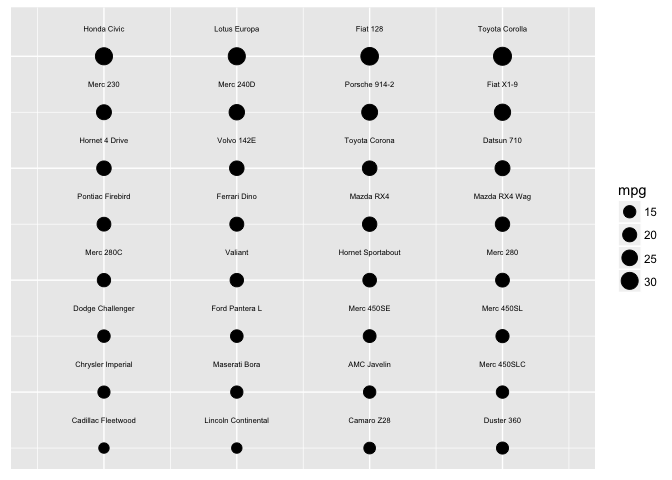
\includegraphics[height=0.8\textheight]{autosarea}
\end{center}
\end{frame}


%---------------------------------------------------------------------------------------------------------------------------------------- 
\begin{frame}{Ordre d'encodage}
La mesure la plus importante devrait exploiter l'encodage ayant le rang le plus haut :
\begin{enumerate}
	\item Position sur une échelle commune
	\item Position sur une échelle identique non alignée
	\item Longueur
	\item \red{Angle ou pente}
	\item Aire
	\item Volume ou Densité ou Saturation de couleur
	\item Teinte de couleur
\end{enumerate}
\end{frame}

%---------------------------------------------------------------------------------------------------------------------------------------- 
\begin{frame}{Exemple d'angle : dataset autos}
\begin{center}
	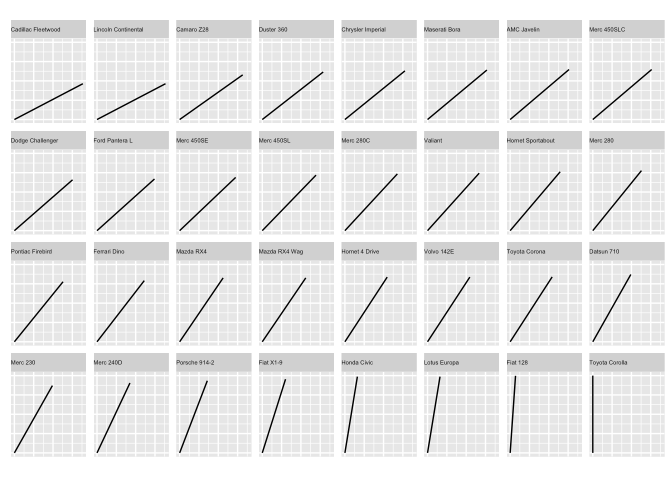
\includegraphics[height=0.8\textheight]{autosangle}
\end{center}
\end{frame}

%---------------------------------------------------------------------------------------------------------------------------------------- 
\begin{frame}{Exemple d'angle : Pop. mondiale}
\begin{center}
	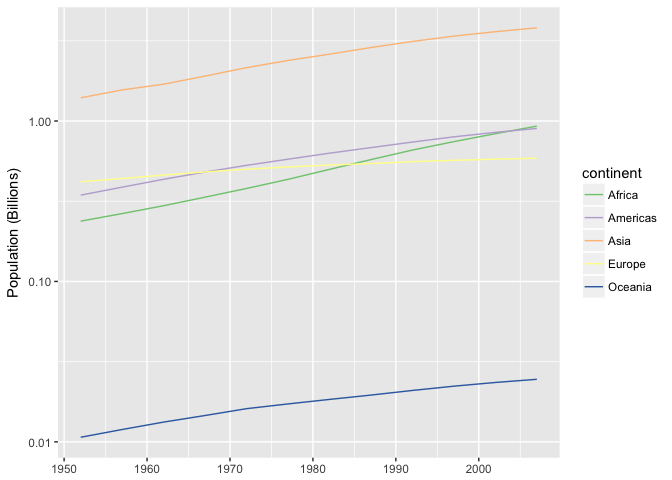
\includegraphics[height=0.8\textheight]{popgrowth}
\end{center}
\end{frame}

%---------------------------------------------------------------------------------------------------------------------------------------- 
\begin{frame}{Ordre d'encodage}
La mesure la plus importante devrait exploiter l'encodage ayant le rang le plus haut :
\begin{enumerate}
	\item Position sur une échelle commune
	\item Position sur une échelle identique non alignée
	\item \red{Longueur}
	\item Angle ou pente
	\item Aire
	\item Volume ou Densité ou Saturation de couleur
	\item Teinte de couleur
\end{enumerate}
\end{frame}

%---------------------------------------------------------------------------------------------------------------------------------------- 
\begin{frame}{Exemple de longueur : dataset autos}
\begin{center}
	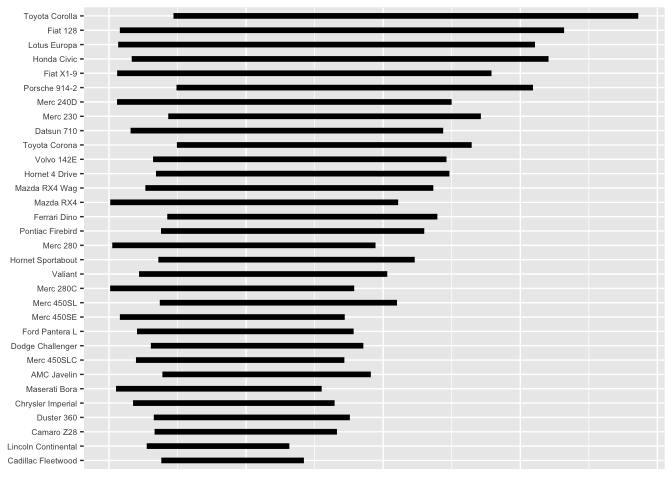
\includegraphics[height=0.8\textheight]{autosline_rand}
\end{center}
\end{frame}

%---------------------------------------------------------------------------------------------------------------------------------------- 
\begin{frame}{Exemple de longueur : quartiles}
\begin{center}
	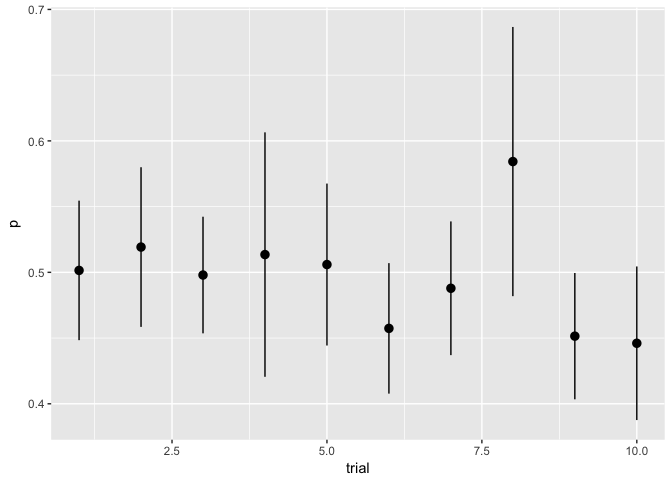
\includegraphics[height=0.8\textheight]{quantiles}
\end{center}
\end{frame}

%---------------------------------------------------------------------------------------------------------------------------------------- 
\begin{frame}{Ordre d'encodage}
La mesure la plus importante devrait exploiter l'encodage ayant le rang le plus haut :
\begin{enumerate}
	\item Position sur une échelle commune
	\item \red{Position sur une échelle identique non alignée}
	\item Longueur
	\item Angle ou pente
	\item Aire
	\item Volume ou Densité ou Saturation de couleur
	\item Teinte de couleur
\end{enumerate}
\end{frame}

%---------------------------------------------------------------------------------------------------------------------------------------- 
\begin{frame}{Exemple de position non alignée : autos}
\begin{center}
	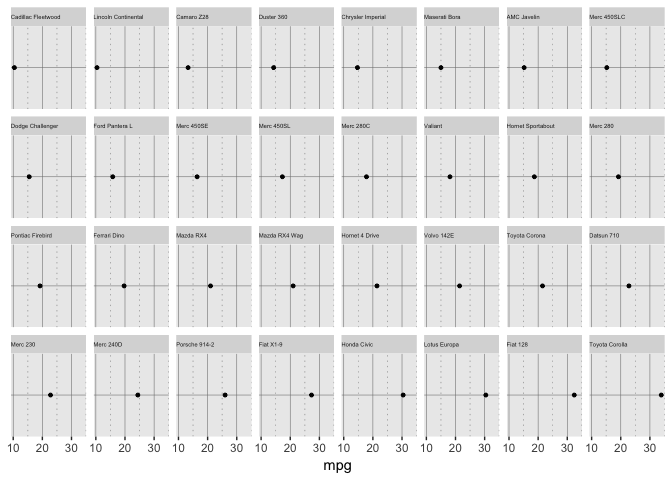
\includegraphics[height=0.8\textheight]{autosloc}
\end{center}
\end{frame}

%---------------------------------------------------------------------------------------------------------------------------------------- 
\begin{frame}{Exemple de position non alignée : latence}
\begin{center}
	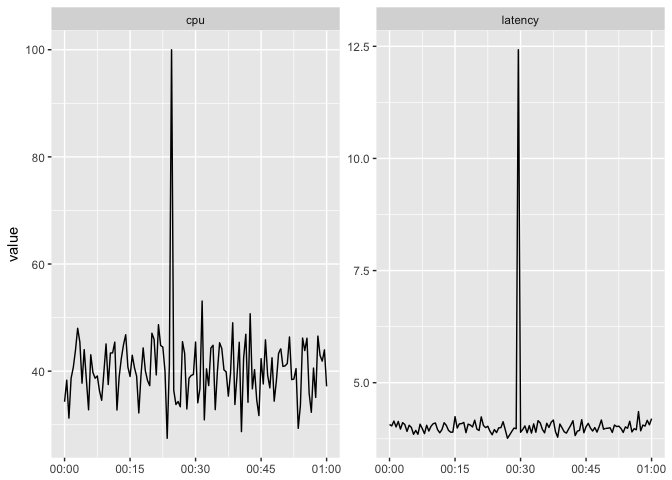
\includegraphics[height=0.8\textheight]{latency}
\end{center}
\end{frame}

%---------------------------------------------------------------------------------------------------------------------------------------- 
\begin{frame}{Ordre d'encodage}
La mesure la plus importante devrait exploiter l'encodage ayant le rang le plus haut :
\begin{enumerate}
	\item \red{Position sur une échelle commune}
	\item Position sur une échelle identique non alignée
	\item Longueur
	\item Angle ou pente
	\item Aire
	\item Volume ou Densité ou Saturation de couleur
	\item Teinte de couleur
\end{enumerate}
\end{frame}

%---------------------------------------------------------------------------------------------------------------------------------------- 
\begin{frame}{Exemple de position alignée : autos}
\begin{center}
	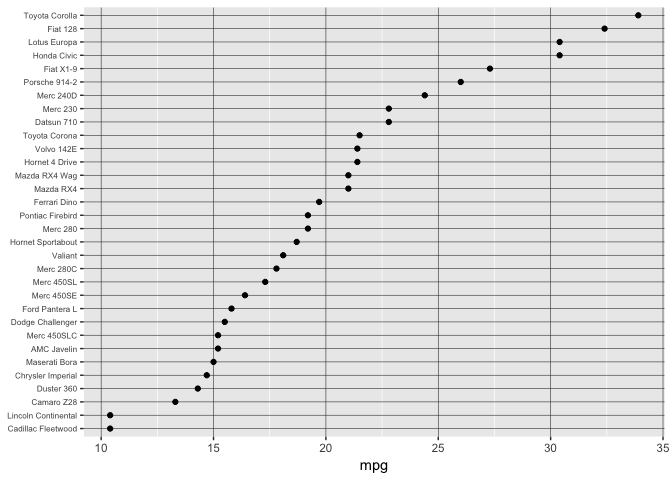
\includegraphics[height=0.8\textheight]{autosloc_order}
\end{center}
\end{frame}


%---------------------------------------------------------------------------------------------------------------------------------------- 
\begin{frame}{Ordre d'encodage}
La mesure la plus importante devrait exploiter l'encodage ayant le rang le plus haut :
\begin{enumerate}
	\item Position sur une échelle commune
	\item Position sur une échelle identique non alignée
	\item Longueur
	\item Angle ou pente
	\item Aire
	\item Volume ou Densité ou Saturation de couleur
	\item Teinte de couleur
\end{enumerate}
\end{frame}


%---------------------------------------------------------------------------------------------------------------------------------------- 
\begin{frame}{Observation}
\begin{center}\begin{Huge}\textbf{
		\red{Empiler} n'importe quoi est quasiment toujours une \red{erreur}.
}\end{Huge}\end{center}
\end{frame}

%---------------------------------------------------------------------------------------------------------------------------------------- 
\begin{frame}{Exemple empilé : dataset diamants}
\begin{center}
	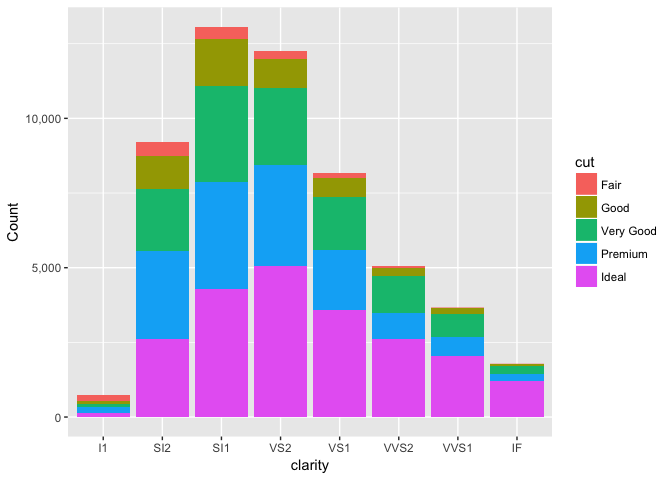
\includegraphics[height=0.8\textheight]{diamonds}
\end{center}
\end{frame}

%---------------------------------------------------------------------------------------------------------------------------------------- 
\begin{frame}{Exemple empilé : dataset diamants}
\begin{center}
	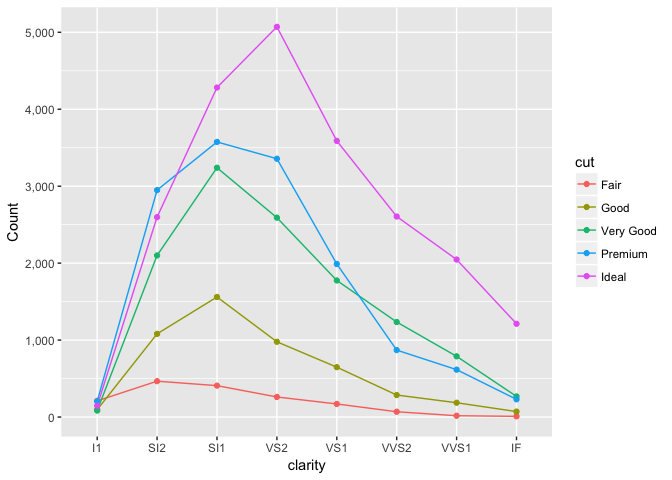
\includegraphics[height=0.8\textheight]{diamonds_type}
\end{center}
\end{frame}

%---------------------------------------------------------------------------------------------------------------------------------------- 
\begin{frame}{Exemple empilé : dataset diamants}
\begin{center}
	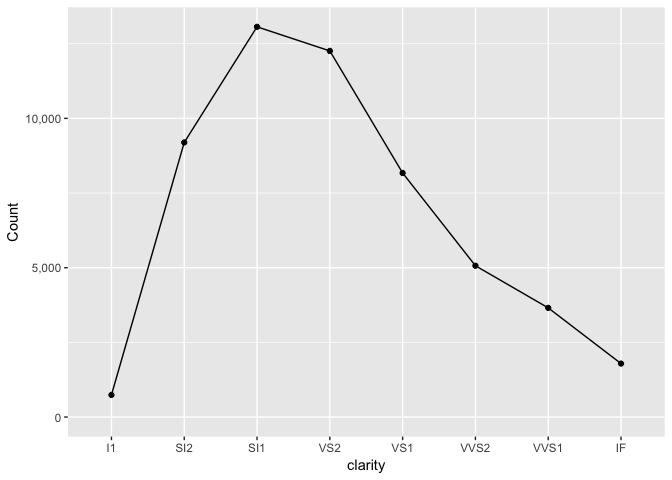
\includegraphics[height=0.8\textheight]{diamonds_sum}
\end{center}
\end{frame}


%---------------------------------------------------------------------------------------------------------------------------------------- 
\begin{frame}{Exemple empilé : dataset diamants}
\begin{minipage}{.45\textwidth}
	\begin{center}
		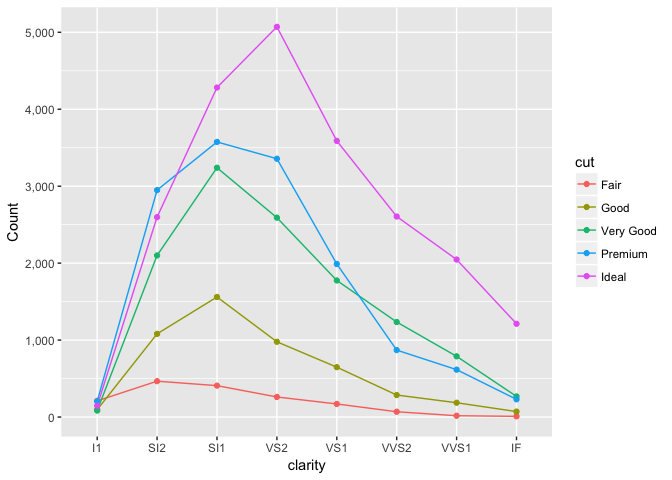
\includegraphics[width=\textwidth]{diamonds_type}
	\end{center}
\end{minipage}
\hfill
\begin{minipage}{.45\textwidth}
	\begin{center}
		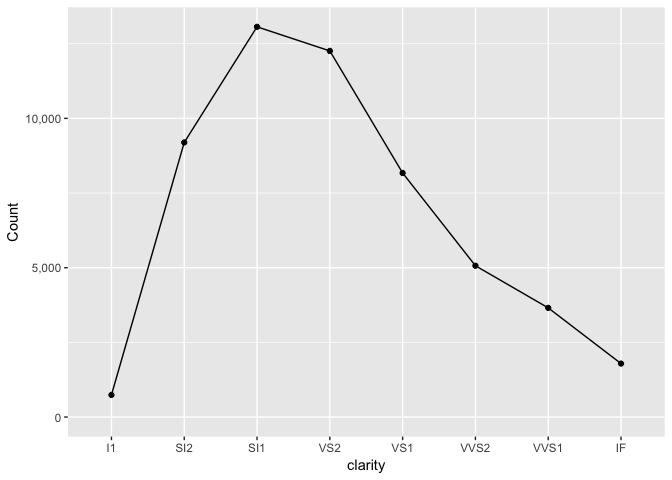
\includegraphics[width=\textwidth]{diamonds_sum}
	\end{center}
\end{minipage}
\end{frame}


%---------------------------------------------------------------------------------------------------------------------------------------- 
\begin{frame}{Observation}
\begin{center}\begin{Huge}\textbf{
			\red{Empiler} provoque une interprétation des \red{longueurs} pas des positions sur une échelle commune.
}\end{Huge}\end{center}
\end{frame}


%---------------------------------------------------------------------------------------------------------------------------------------- 
\begin{frame}{Observation}
\begin{center}\begin{Huge}\textbf{
			Empiler n'importe quoi est \red{quasiment} toujours une erreur.
}\end{Huge}\end{center}
\end{frame}

%---------------------------------------------------------------------------------------------------------------------------------------- 
\begin{frame}{Exemple empilé : dataset OS market}
\begin{center}
	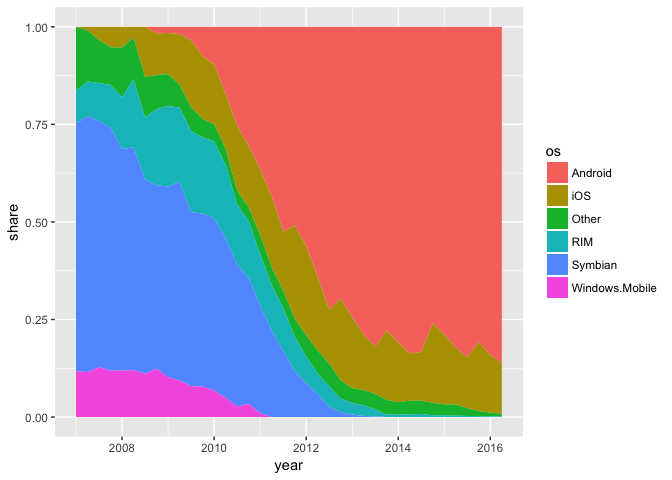
\includegraphics[height=0.8\textheight]{os}
\end{center}
\end{frame}

%---------------------------------------------------------------------------------------------------------------------------------------- 
\begin{frame}{Observation}
\begin{center}\begin{Huge}\textbf{
			Les \emph{pie charts} sont \red{TOUJOURS} une erreur.
}\end{Huge}\end{center}
\end{frame}

%---------------------------------------------------------------------------------------------------------------------------------------- 
\begin{frame}{Citation}
\begin{center}\begin{large}\textbf{
			"Pie charts are the information visualization equivalent of a roofing hammer to the frontal lobe."
}\end{large}\end{center}

Les camemberts sont l'équivalent visuel d'un coup de marteau sur le lobe frontal.

\vspace{1cm}
- Coda Hale
\end{frame}

%---------------------------------------------------------------------------------------------------------------------------------------- 
\begin{frame}{\emph{Pie Charts}}
La mesure la plus importante devrait exploiter l'encodage ayant le rang le plus haut :
\begin{enumerate}
	\item Position sur une échelle commune
	\item Position sur une échelle identique non alignée
	\item Longueur
	\item \red{Angle ou pente}
	\item Aire
	\item Volume ou Densité ou Saturation de couleur
	\item Teinte de couleur
\end{enumerate}
\end{frame}

%---------------------------------------------------------------------------------------------------------------------------------------- 
\begin{frame}{Exemple de pie chart : 2016 US election web poll}
\begin{center}
	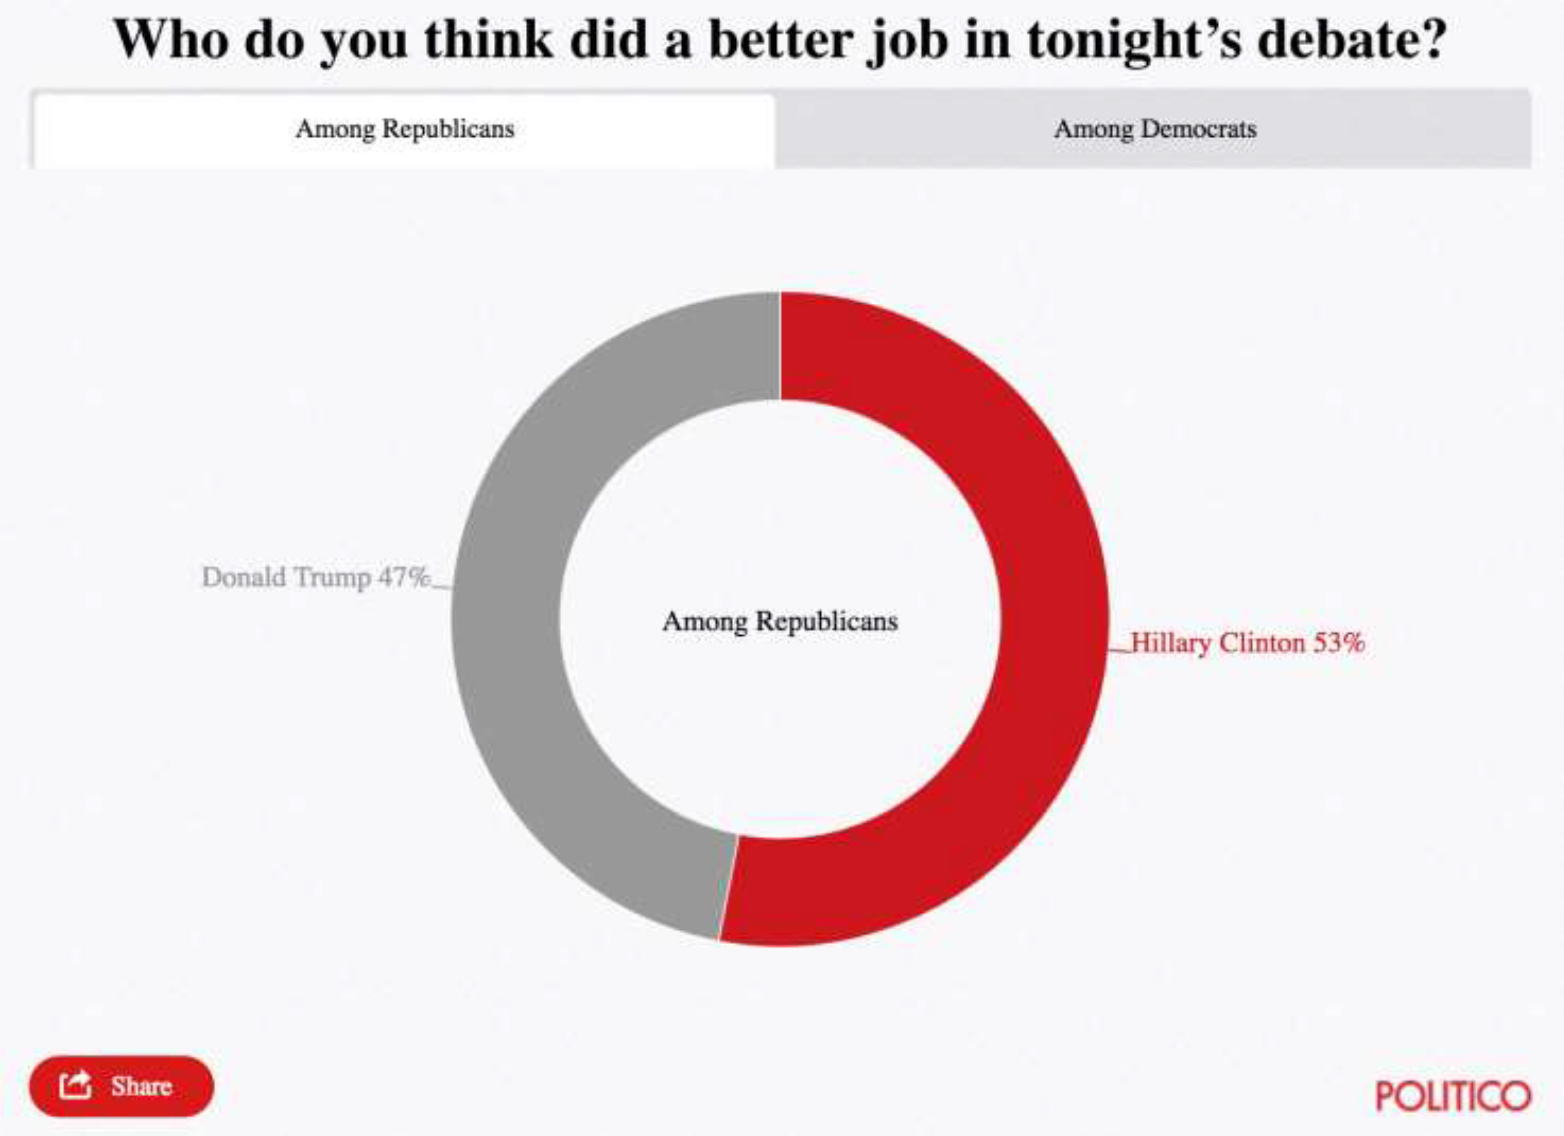
\includegraphics[height=0.8\textheight]{rep}
\end{center}
\end{frame}

%---------------------------------------------------------------------------------------------------------------------------------------- 
\begin{frame}{Exemple de pie chart : 2016 US election web poll}
\begin{center}
	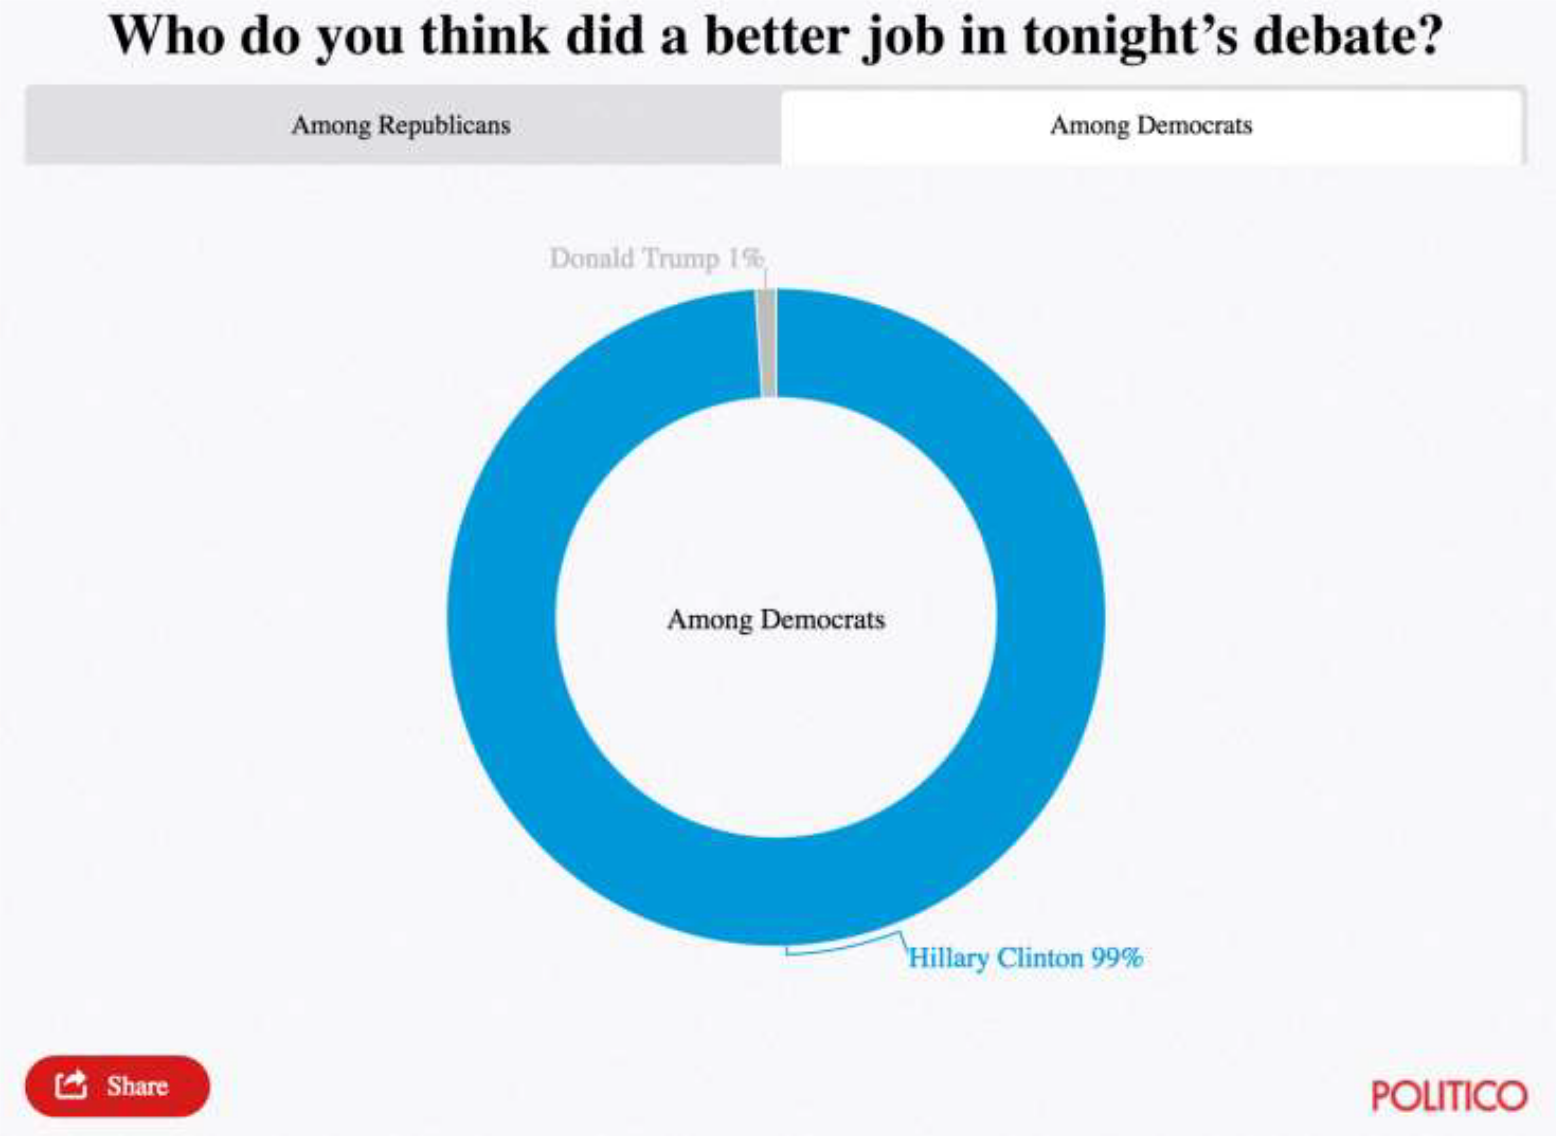
\includegraphics[height=0.8\textheight]{dem}
\end{center}
\end{frame}

%---------------------------------------------------------------------------------------------------------------------------------------- 
\begin{frame}{Citation}
	\red{Tables are preferable to graphics for many small data sets.}\\ A table is nearly always better than a dumb pie chart; the only thing worse than a pie chart is several of them, for then the viewer is asked to compared quantities located in spatial disarray both within and between pies… Given their low data-density and failure to order numbers along a visual dimension, pie charts should never be used.

\vspace{1cm}
-Edward Tufte, The Visual Display of Quantitative Information

\end{frame}

%---------------------------------------------------------------------------------------------------------------------------------------- 
\begin{frame}{Exemple de pie chart : 2016 US election web poll}
\begin{center}
	Qui pensez vous a fait un meilleur débat ? 
	
	\vspace{.5cm}
	\begin{tabular}{|c|c|c|}
		\hline 
		& Clinton & Trump \\ 
		\hline 
		Démocrates & 99\% & 1\% \\ 
		\hline 
		Républicains & 53\% & 47\% \\ 
		\hline 
	\end{tabular} 
\end{center}
\end{frame}

%---------------------------------------------------------------------------------------------------------------------------------------- 
\begin{frame}{Observation}
\begin{center}\begin{Huge}\textbf{
			Les bons \emph{pie charts} sont des \red{blagues}.
}\end{Huge}\end{center}
\end{frame}


%---------------------------------------------------------------------------------------------------------------------------------------- 
\begin{frame}{Exemple de pie chart égyptien}
\begin{center}
	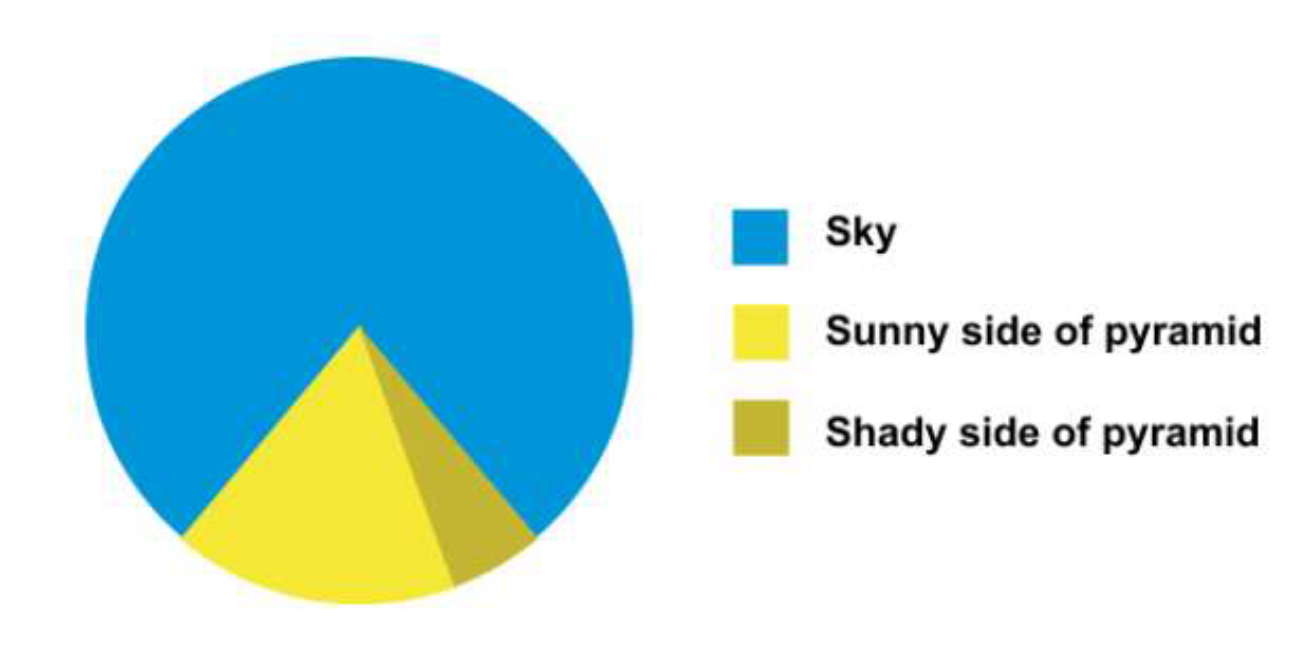
\includegraphics[width=\textwidth]{pie}
\end{center}
\end{frame}

%---------------------------------------------------------------------------------------------------------------------------------------- 
\begin{frame}{Observation}
\begin{center}\begin{Huge}\textbf{
			La comparaison est triviale sur une \red{échelle commune}
}\end{Huge}\end{center}
\end{frame}

%---------------------------------------------------------------------------------------------------------------------------------------- 
\begin{frame}{Exemple de comparaison : latence}
\begin{center}
	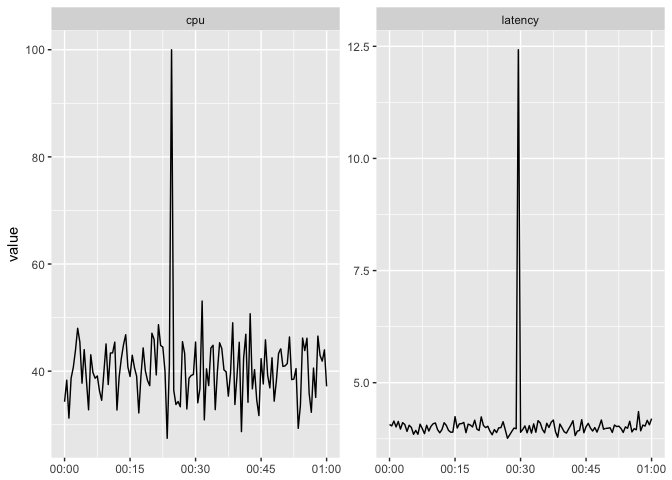
\includegraphics[width=\textwidth]{latency}
\end{center}
\end{frame}

%---------------------------------------------------------------------------------------------------------------------------------------- 
\begin{frame}{Exemple de comparaison : latence}
\begin{center}
	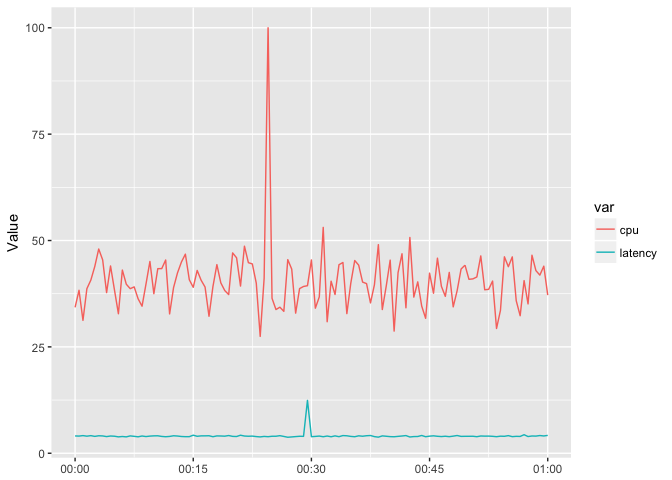
\includegraphics[width=\textwidth]{latency2}
\end{center}
\end{frame}

%---------------------------------------------------------------------------------------------------------------------------------------- 
\begin{frame}{Exemple de comparaison : latence}
\begin{center}
	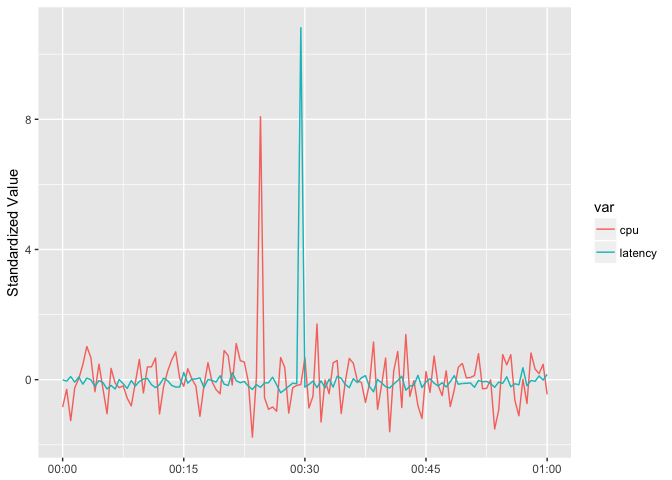
\includegraphics[width=\textwidth]{latency3}
\end{center}
\end{frame}

%---------------------------------------------------------------------------------------------------------------------------------------- 
\begin{frame}{Observation}
\begin{center}\begin{Huge}\textbf{
			Les \emph{scatters plots} montrent les \red{relations} directement.
}\end{Huge}\end{center}
\end{frame}

%---------------------------------------------------------------------------------------------------------------------------------------- 
\begin{frame}{Exemple de \emph{scatters plots} : latence}
\begin{center}
	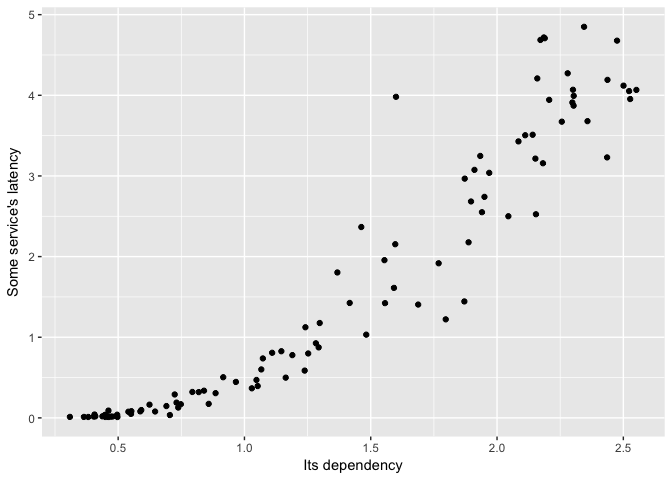
\includegraphics[width=\textwidth]{latency_sp}
\end{center}
\end{frame}

%---------------------------------------------------------------------------------------------------------------------------------------- 
\begin{frame}{Exemple de \emph{scatters plots} : latence}
\begin{center}
	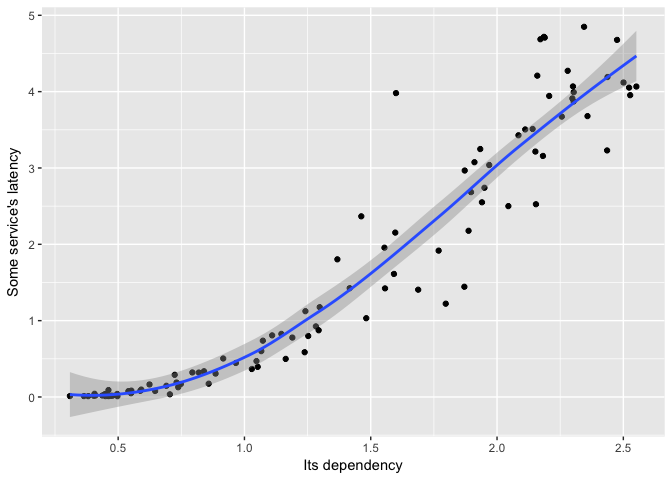
\includegraphics[width=\textwidth]{latency_sp2}
\end{center}
\end{frame}

%---------------------------------------------------------------------------------------------------------------------------------------- 
\begin{frame}{Observation}
\begin{center}\begin{Huge}\textbf{
			Les graphes de croissance \red{n'en sont pas} (usuellement).
}\end{Huge}\end{center}
\end{frame}

%---------------------------------------------------------------------------------------------------------------------------------------- 
\begin{frame}{Exemple de \emph{growth chart} : Pop. mondiale}
\begin{center}
	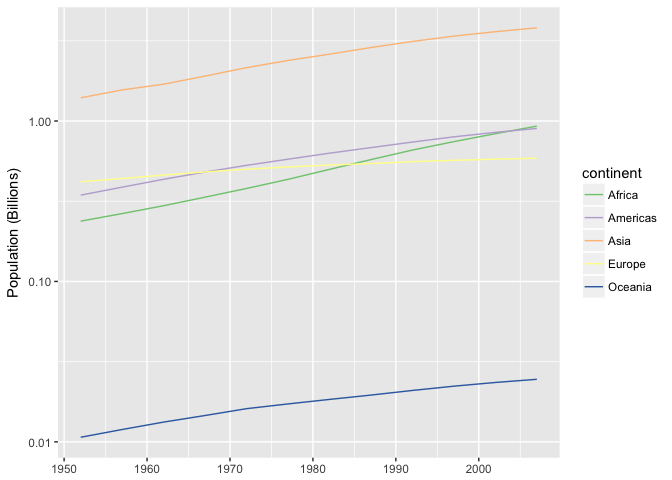
\includegraphics[width=\textwidth]{popgrowth}
\end{center}
\end{frame}

%---------------------------------------------------------------------------------------------------------------------------------------- 
\begin{frame}{Observation}
\begin{center}\begin{Huge}\textbf{
			Si la croissance (pente/dérivée)\\
			est importante,\\			
			\red{affichez-la directement}
}\end{Huge}\end{center}
\end{frame}

%---------------------------------------------------------------------------------------------------------------------------------------- 
\begin{frame}{Exemple de \emph{growth chart} : Pop. mondiale}
\begin{center}
	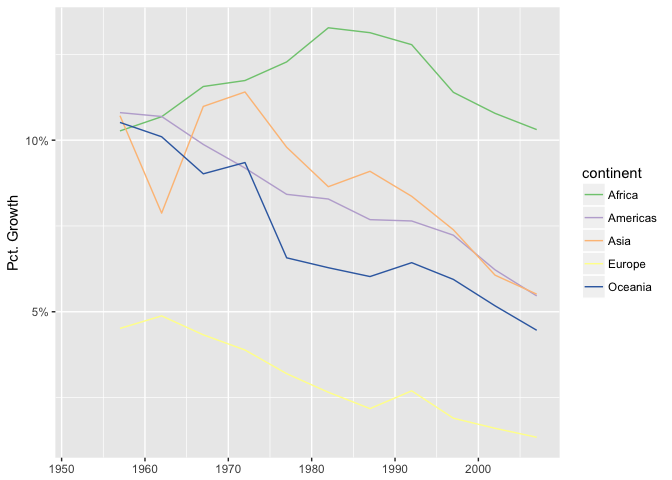
\includegraphics[width=\textwidth]{popgrowth_real}
\end{center}
\end{frame}

%---------------------------------------------------------------------------------------------------------------------------------------- 
\begin{frame}{À retenir pour l'estimation : Ordre d'encodage}
La mesure la plus importante devrait exploiter l'encodage ayant le rang le plus haut :
\begin{enumerate}
	\item Position sur une échelle commune
	\item Position sur une échelle identique non alignée
	\item Longueur
	\item Angle ou pente
	\item Aire
	\item Volume ou Densité ou Saturation de couleur
	\item Teinte de couleur
\end{enumerate}
\end{frame}

\section*{Construction}
%---------------------------------------------------------------------------------------------------------------------------------------- 
\begin{frame}{Outline}
Trois opérations visuelles dans la perception de shémas : 
\begin{enumerate}
	\item Détection
	\item \red{Construction}
	\item Estimation
\end{enumerate}
\end{frame}


%---------------------------------------------------------------------------------------------------------------------------------------- 
\begin{frame}{Construction}
Principes d'organisation implicite :
\begin{enumerate}
	\item Réification
	\item Émrgence
	\item Prägnanz : Concis et plein de sens
	\begin{enumerate}
		\item Fermeture
		\item Continuation
		\item Proximité
		\item Similarité
	\end{enumerate}
\end{enumerate}
\end{frame}


%---------------------------------------------------------------------------------------------------------------------------------------- 
\begin{frame}{Réification}
\begin{center}
	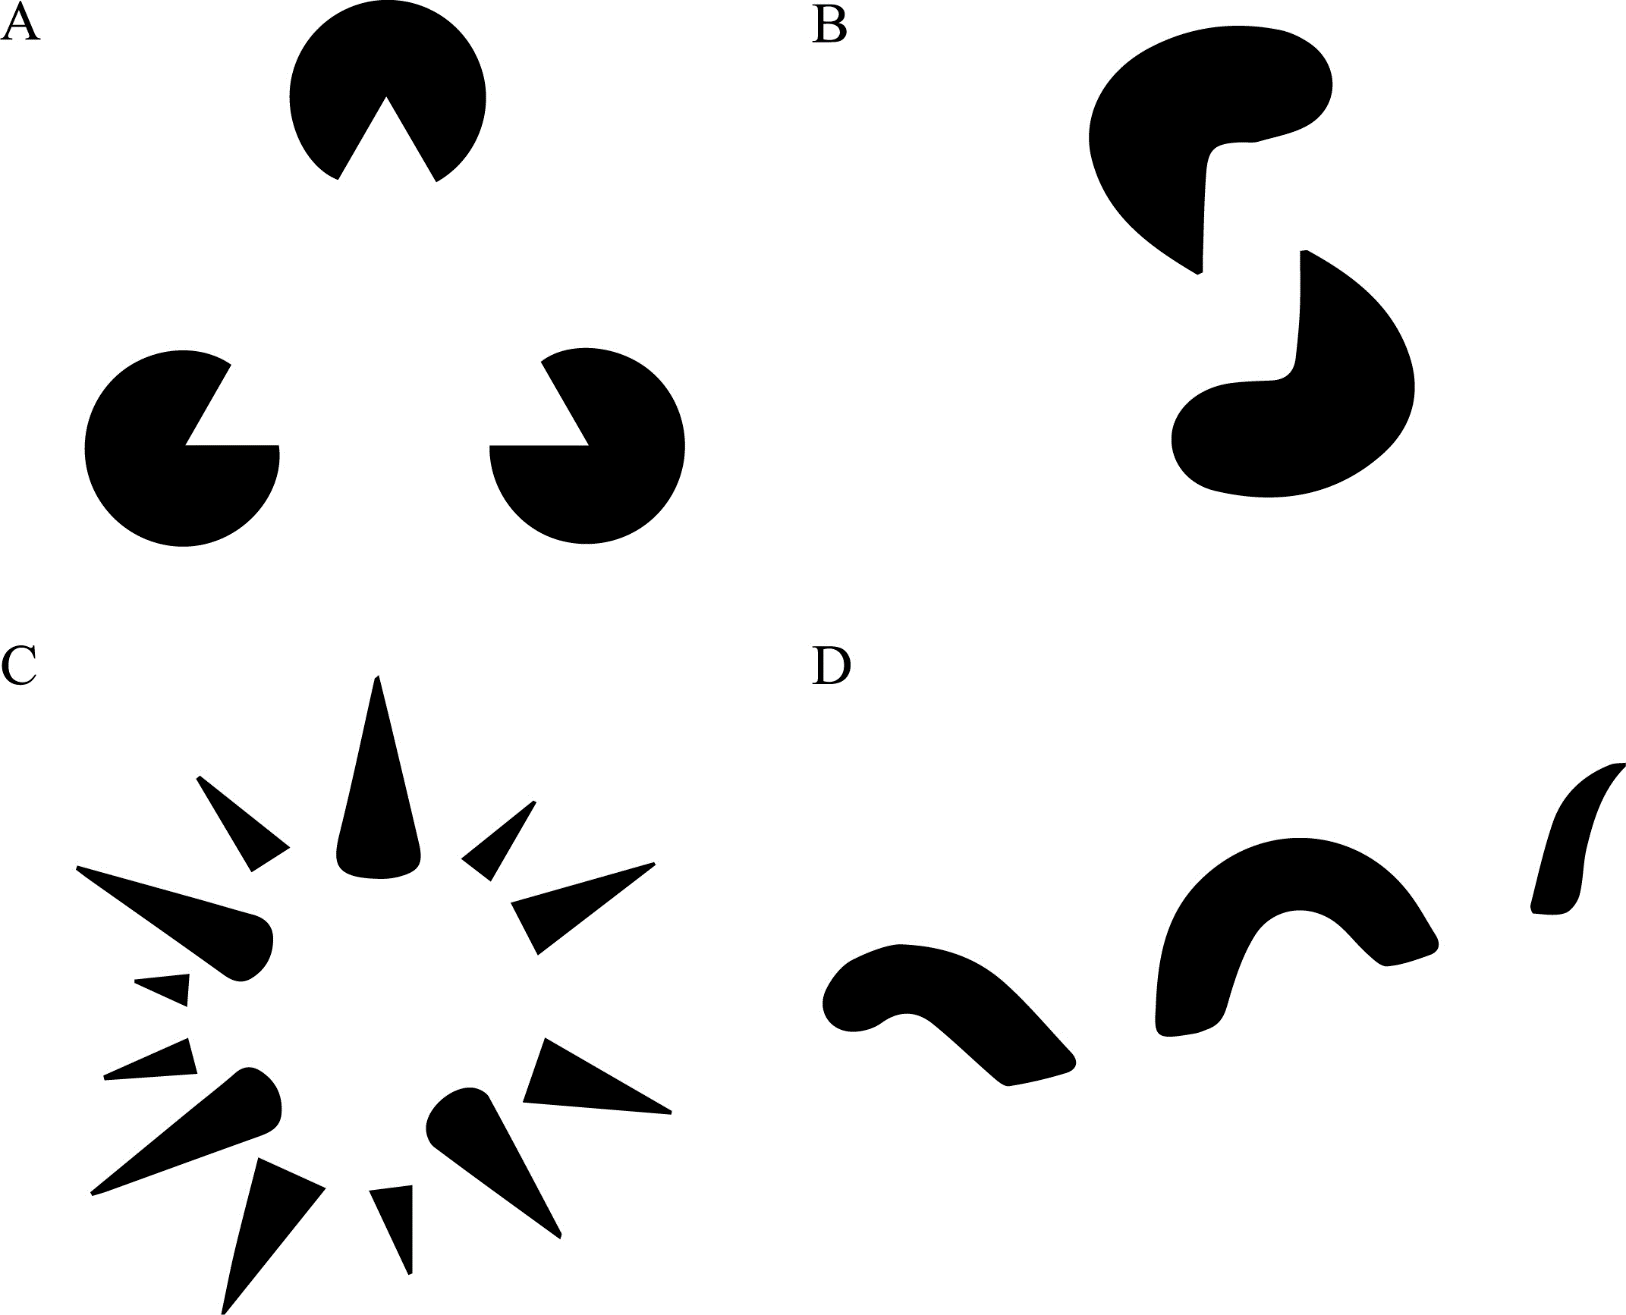
\includegraphics[height=0.8\textheight]{reification}
\end{center}
\flushright{\footnotesize{Source : \url{https://en.wikipedia.org/wiki/Gestalt_psychology}}}
\end{frame}

%---------------------------------------------------------------------------------------------------------------------------------------- 
\begin{frame}{Émergence}
\begin{center}
	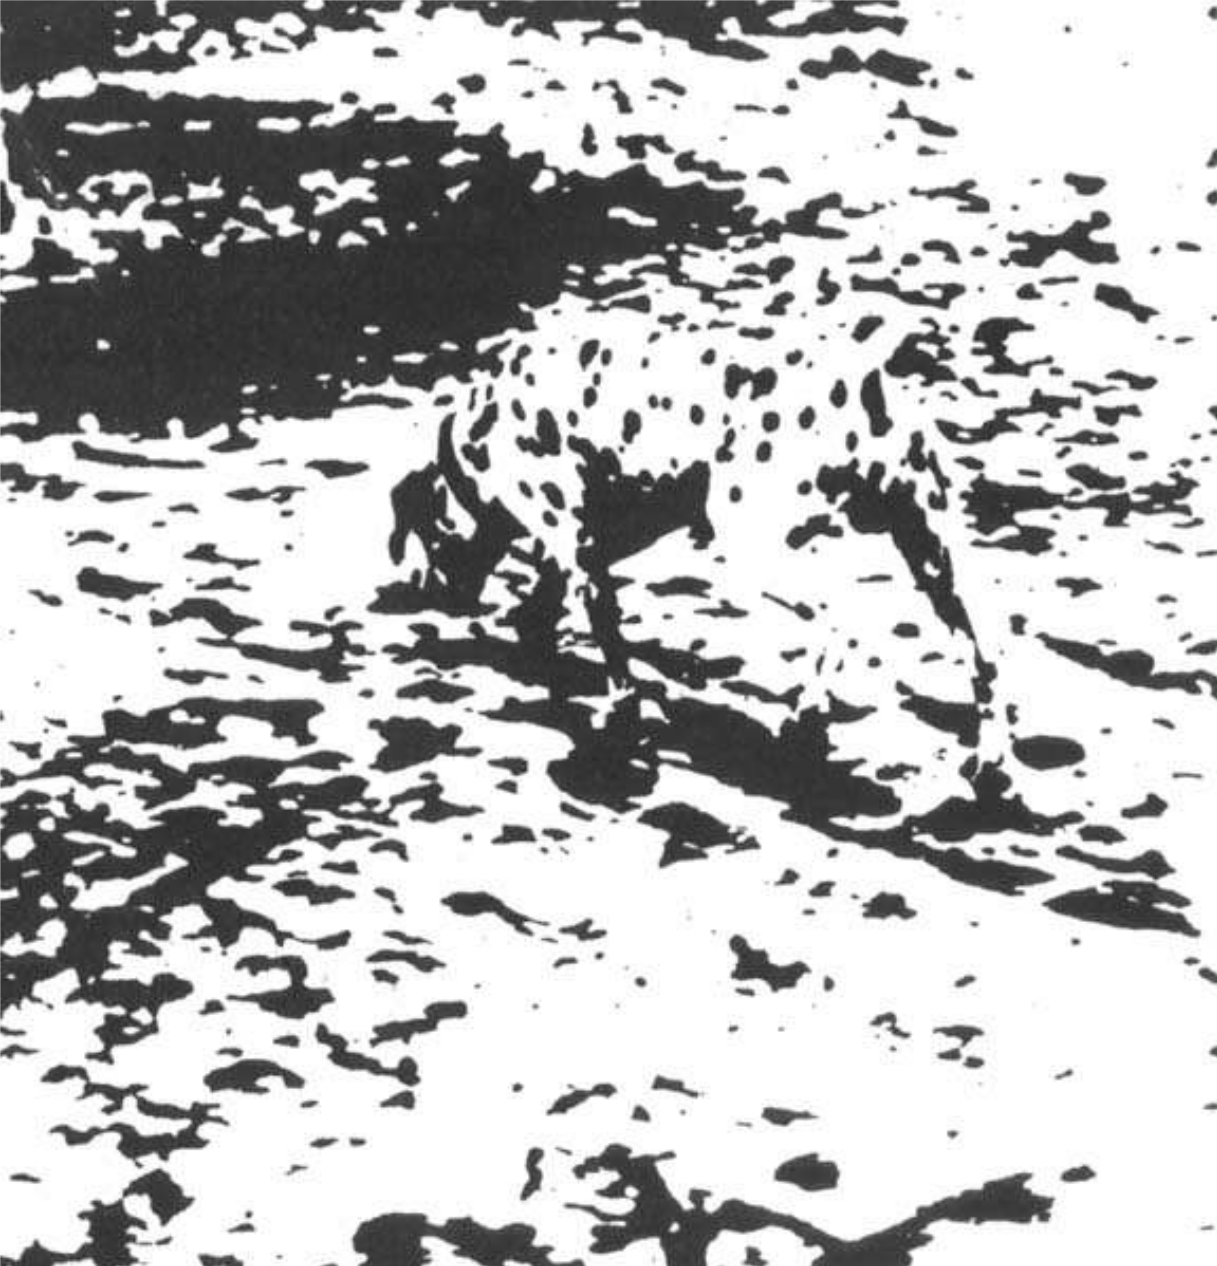
\includegraphics[height=0.8\textheight]{dalmatien}
\end{center}
\flushright{\footnotesize{Source : \url{https://en.wikipedia.org/wiki/Gestalt_psychology}}}
\end{frame}

%---------------------------------------------------------------------------------------------------------------------------------------- 
\begin{frame}{Émergence}
\begin{center}
	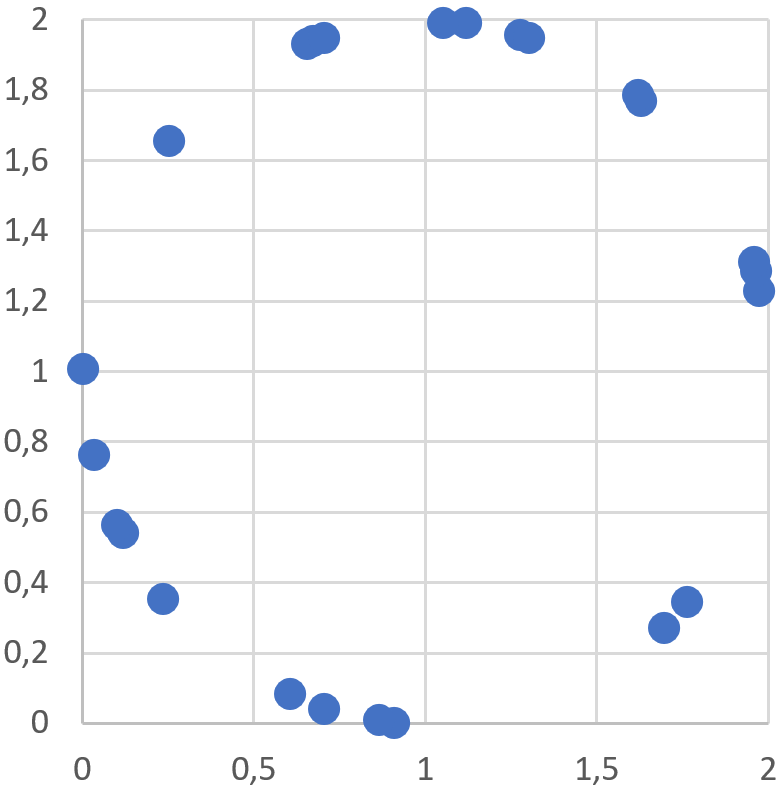
\includegraphics[height=0.8\textheight]{circle}
\end{center}
\end{frame}

%---------------------------------------------------------------------------------------------------------------------------------------- 
\begin{frame}{Prägnanz}
\begin{center}
	\begin{tikzpicture}
		\node(f) at (0,0)
				{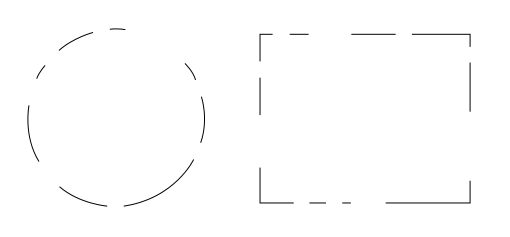
\includegraphics[height=0.25\textheight]{prananz_ferm}};
		\node[align=center,above] at (f.north) {Fermeture};
		\node(s) at (6,0)
				{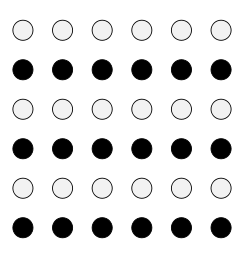
\includegraphics[height=0.25\textheight]{prananz_sim}};
		\node[align=center,above] at (s.north) {Similarité};
		\node(p) at (0,4)
				{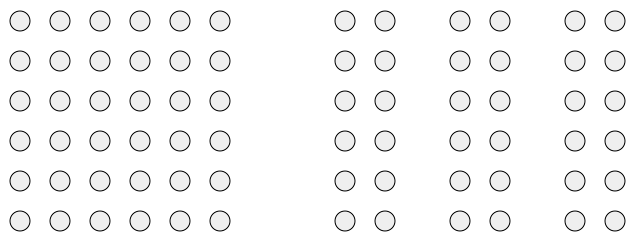
\includegraphics[height=0.25\textheight]{prananz_prox}};
		\node[align=center,below] at (p.south) {Proximité};
		\node(c) at (6,4)
				{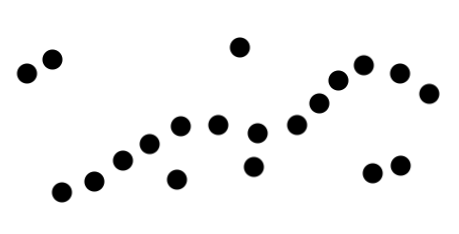
\includegraphics[height=0.25\textheight]{prananz_cont}};
		\node[align=center,below] at (c.south) {Continuité};
	\end{tikzpicture}
\end{center}
\end{frame}

%---------------------------------------------------------------------------------------------------------------------------------------- 
\begin{frame}{Fermeture}
\begin{center}
	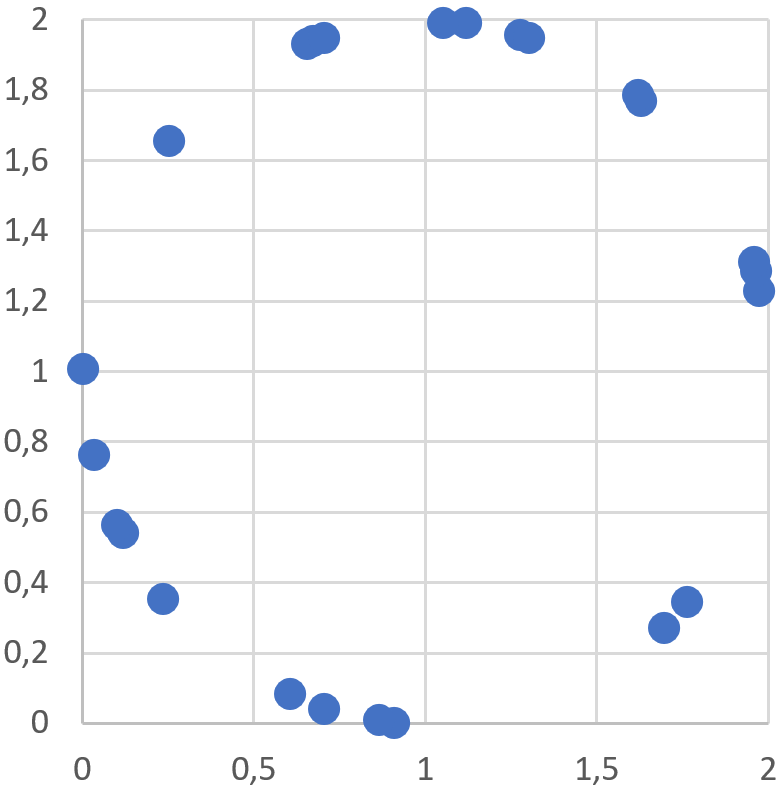
\includegraphics[height=0.8\textheight]{circle}
\end{center}
\end{frame}

%---------------------------------------------------------------------------------------------------------------------------------------- 
\begin{frame}{Continuité}
\begin{center}
	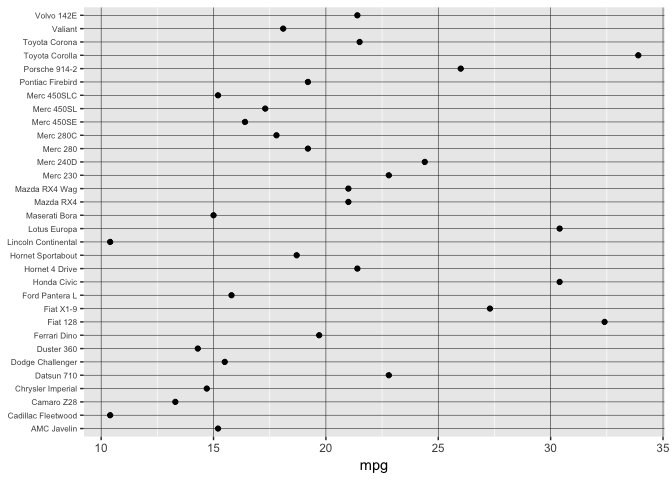
\includegraphics[height=0.8\textheight]{autosloc_rand}
\end{center}
\end{frame}

%---------------------------------------------------------------------------------------------------------------------------------------- 
\begin{frame}{Continuité}
\begin{center}
	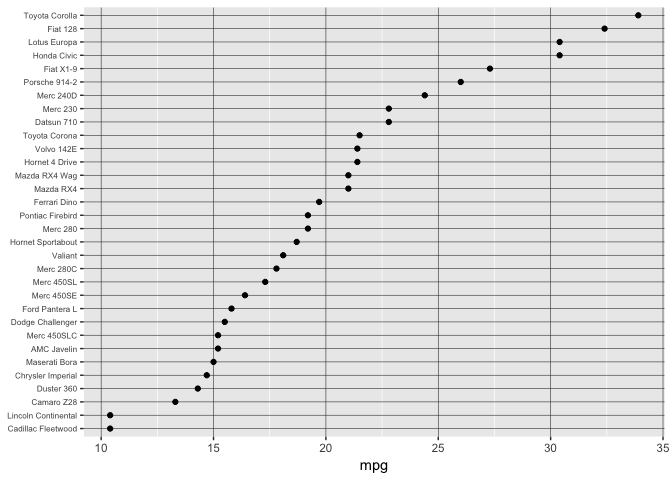
\includegraphics[height=0.8\textheight]{autosloc_order}
\end{center}
\end{frame}

%---------------------------------------------------------------------------------------------------------------------------------------- 
\begin{frame}{Observation}
\begin{center}\begin{Huge}\textbf{
			Les bons graphiques avantagent la \red{continuité} pour améliorer la \red{construction}.
}\end{Huge}\end{center}
\end{frame}


%---------------------------------------------------------------------------------------------------------------------------------------- 
\begin{frame}{Similarité}
\begin{center}\begin{Huge}\textbf{
			Loi de similarité
}\end{Huge}\end{center}
\end{frame}

%---------------------------------------------------------------------------------------------------------------------------------------- 
\begin{frame}{Similarité}
\begin{center}
	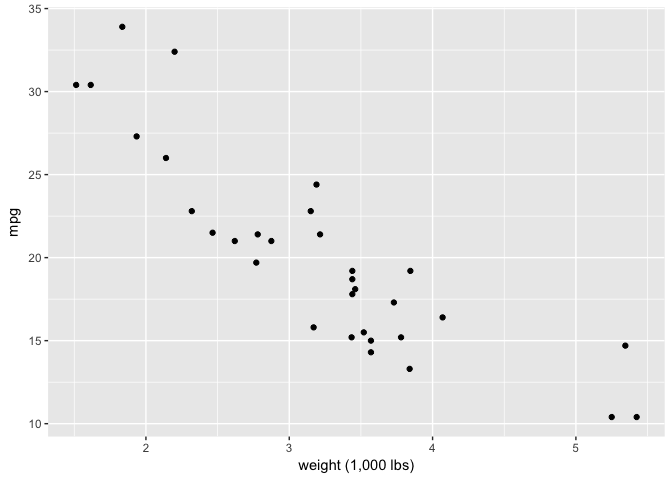
\includegraphics[height=0.8\textheight]{sim}
\end{center}
\end{frame}

%---------------------------------------------------------------------------------------------------------------------------------------- 
\begin{frame}{Similarité}
\begin{center}
	\includegraphics[height=0.8\textheight]{sim2}
\end{center}
\end{frame}

%---------------------------------------------------------------------------------------------------------------------------------------- 
\begin{frame}{Similarité}
\begin{center}
	\includegraphics[height=0.8\textheight]{sim3}
\end{center}
\end{frame}

%---------------------------------------------------------------------------------------------------------------------------------------- 
\begin{frame}{Similarité}
\begin{center}
	\includegraphics[height=0.8\textheight]{sim4}
\end{center}
\end{frame}

%---------------------------------------------------------------------------------------------------------------------------------------- 
\begin{frame}{Similarité}
\begin{center}
	\includegraphics[height=0.8\textheight]{sim5}
\end{center}
\end{frame}

%---------------------------------------------------------------------------------------------------------------------------------------- 
\begin{frame}{Similarité}
\begin{center}
	\includegraphics[height=0.8\textheight]{sim6}
\end{center}
\end{frame}

%---------------------------------------------------------------------------------------------------------------------------------------- 
\begin{frame}{Similarité}
\begin{center}
	\includegraphics[height=0.8\textheight]{sim7}
\end{center}
\end{frame}

%---------------------------------------------------------------------------------------------------------------------------------------- 
\begin{frame}{Proximité}
\begin{center}\begin{Huge}\textbf{
			Loi de proximité
}\end{Huge}\end{center}
\end{frame}

%---------------------------------------------------------------------------------------------------------------------------------------- 
\begin{frame}{Proximité}
\begin{center}
	\includegraphics[height=0.8\textheight]{diamonds_bat}
\end{center}
\end{frame}

%---------------------------------------------------------------------------------------------------------------------------------------- 
\begin{frame}{Proximité}
\begin{center}
	\includegraphics[height=0.8\textheight]{diamonds_type}
\end{center}
\end{frame}

%---------------------------------------------------------------------------------------------------------------------------------------- 
\begin{frame}{Observation}
\begin{center}\begin{Huge}\textbf{
			Les diagrammes en bâtons sont usuellement une \red{mauvaise} idée.
}\end{Huge}\end{center}
\end{frame}


\section*{Detection}
%---------------------------------------------------------------------------------------------------------------------------------------- 
\begin{frame}{}
Trois opérations visuelles dans la perception de shémas : 
\begin{enumerate}
	\item \red{Détection}
	\item Construction
	\item Estimation
\end{enumerate}
\end{frame}

%---------------------------------------------------------------------------------------------------------------------------------------- 
\begin{frame}{Détection}
\begin{center}
	\includegraphics[height=0.8\textheight]{det}
\end{center}
\end{frame}

%---------------------------------------------------------------------------------------------------------------------------------------- 
\begin{frame}{Détection}
\begin{center}
	\includegraphics[height=0.8\textheight]{det2}
\end{center}
\end{frame}

%---------------------------------------------------------------------------------------------------------------------------------------- 
\begin{frame}{Détection}
\begin{center}
	\includegraphics[height=0.8\textheight]{det3}
\end{center}
\end{frame}

%---------------------------------------------------------------------------------------------------------------------------------------- 
\begin{frame}{Détection}
\begin{center}
	\includegraphics[height=0.8\textheight]{det4}
\end{center}
\end{frame}

%---------------------------------------------------------------------------------------------------------------------------------------- 
\begin{frame}{Détection}
\begin{center}
	\includegraphics[height=0.8\textheight]{det5}
\end{center}
\end{frame}

%---------------------------------------------------------------------------------------------------------------------------------------- 
\begin{frame}{Détection}
\begin{center}
	\includegraphics[height=0.8\textheight]{det6}
\end{center}
\end{frame}


%---------------------------------------------------------------------------------------------------------------------------------------- 
\begin{frame}{Détection}
\begin{center}\begin{Huge}\textbf{
			La détection n'est pas aussi triviale qu'elle ne paraît.
}\end{Huge}\end{center}
\end{frame}

%---------------------------------------------------------------------------------------------------------------------------------------- 
\begin{frame}{Détection}
\begin{center}
	\includegraphics[height=0.8\textheight]{det7}
\end{center}
\end{frame}

%---------------------------------------------------------------------------------------------------------------------------------------- 
\begin{frame}{}
\begin{Large}
	"Avant tout, montrez les données."
	
	\vspace{1cm}
	\textit{- Tufte}
\end{Large}
\end{frame}

\section{Autres résultats utiles}

%---------------------------------------------------------------------------------------------------------------------------------------- 
\begin{frame}{Loi de Weber}
\begin{center}\begin{huge}\textbf{
			La "différence juste notable" est \red{proportionnel} à la taille du stimuli initial.
}\end{huge}\end{center}
\end{frame}

%---------------------------------------------------------------------------------------------------------------------------------------- 
\begin{frame}{Loi de Weber}
\begin{center}
	\resizebox{\textwidth}{!}{
	\begin{tikzpicture}
	\only<1->{
		\filldraw[fill=ulred] (9,0.2)rectangle +(1,1) node[pos=.5] {10};
		\filldraw[fill=ulred] (11,0) rectangle +(1.414,1.414) node[pos=.5] {20};
		\fill[fill=white] (0,-10.75) rectangle +(10,10);
		\fill[fill=white] (11,-11) rectangle +(10.488,10.488);
	}
	\only<2>{	
		\filldraw[fill=ulred] (0,-10.76) rectangle +(10,10) node[pos=.5] {100};
		\filldraw[fill=ulred] (11,-11) rectangle +(10.488,10.488) node[pos=.5] {110};
	}
	\end{tikzpicture}}
\end{center}
\end{frame}


%---------------------------------------------------------------------------------------------------------------------------------------- 
\begin{frame}{Loi de Weber}
\begin{center}
	\resizebox{!}{0.8\textheight}{
	\begin{tikzpicture}
	\only<1->{
		\filldraw[fill=ulred] (0,0) rectangle +(1,10.3);
		\filldraw[fill=ulred] (4,1) rectangle +(1,10);
		\fill[fill=white] (0,10.305) rectangle +(1,1.7);
		\fill[fill=white] (4,11.005) rectangle +(1,2);
	}
	\only<2>{	
		\filldraw[fill=ulgold] (0,10.305) rectangle +(1,1.7);
		\filldraw[fill=ulgold] (4,11.005) rectangle +(1,2);
		
		\draw[<->,very thick] (1.5,0) -- +(0,12) node[midway,right]{12 cm};
		\draw[<->,very thick] (5.5,1) -- +(0,12) node[midway,right]{12 cm};
	}
	\end{tikzpicture}}
\end{center}
\end{frame}





%---------------------------------------------------------------------------------------------------------------------------------------- 
\begin{frame}{Loi de Weber}
\begin{center}\begin{Huge}\textbf{
			La loi de Weber est la raison de l'utilité des grilles de fond.
}\end{Huge}\end{center}
\end{frame}

%---------------------------------------------------------------------------------------------------------------------------------------- 
\begin{frame}{Loi de Weber}
\begin{center}
	\begin{minipage}{.49\textwidth}
		\begin{center}
			\begin{tikzpicture}
				\node[anchor=south west] at (0,0) {\includegraphics[width=\textwidth]{weber_sans}};
\only<2>{
				\draw[<-,ulgold,ultra thick] (.4,3.5) -- +(.5,-.5);
				\draw[<-,ulgold,ultra thick] (3.2,1.5) -- +(.5,-.5);				
}			\end{tikzpicture}
		\end{center}
	\end{minipage}
	\hfill
	\begin{minipage}{.49\textwidth}
		\begin{center}
\only<3>{\includegraphics[width=\textwidth]{weber_avec}}
		\end{center}
	\end{minipage}

\end{center}
\end{frame}


%---------------------------------------------------------------------------------------------------------------------------------------- 
\begin{frame}{}
\begin{Large}
	"Effacez tout ce qui n'est pas des données."
	
	\vspace{1cm}
	\textit{- Tufte}
\end{Large}
\end{frame}

%---------------------------------------------------------------------------------------------------------------------------------------- 
\begin{frame}{}
\begin{Large}
	"Effacez tout ce qui n'est pas des données \red{avec une bonne raison}."
	
	\vspace{1cm}
	\textit{- Tufte}
\end{Large}
\end{frame}

%---------------------------------------------------------------------------------------------------------------------------------------- 
\begin{frame}{}
\begin{Large}
	"Effacez tout ce qui n'est pas des données et qui interfère avec la détection, la construction ou l'estimation."
	
	\vspace{1cm}
	\textit{- Rause (via Tufte)}
\end{Large}
\end{frame}

%---------------------------------------------------------------------------------------------------------------------------------------- 
\begin{frame}{Observation}
\begin{Large}
	Vous êtes meilleur pour détecter les variations de pente autour de 45 degrés.
\end{Large}
\end{frame}

%---------------------------------------------------------------------------------------------------------------------------------------- 
\begin{frame}{Pente}
\begin{center}
		\begin{tikzpicture}
			\node[anchor=south west] at (0,0) {\includegraphics[width=.5\textwidth]{pente_flat}};
			\node[anchor=south west] at (6,0) {\includegraphics[width=.5\textwidth]{pente_vert}};
			\uncover<2>{\node[anchor=south west] at (3,3) {\includegraphics[width=.5\textwidth]{pente_45}};}		
		\end{tikzpicture}
\end{center}
\end{frame}

%---------------------------------------------------------------------------------------------------------------------------------------- 
\begin{frame}{Observation}
\begin{Large}
	Juste autour de 45$^o$ montre les meilleurs variations de pente.
\end{Large}
\end{frame}

%---------------------------------------------------------------------------------------------------------------------------------------- 
\begin{frame}{Pente}
\begin{center}
	\includegraphics[height=0.8\textheight]{signal_dense}
\end{center}
\end{frame}

%---------------------------------------------------------------------------------------------------------------------------------------- 
\begin{frame}{Pente}
\begin{center}
	\includegraphics[height=0.8\textheight]{signal_45}
\end{center}
\end{frame}

%---------------------------------------------------------------------------------------------------------------------------------------- 
\begin{frame}{Question}
\begin{Large}
	Doit-on inclure 0 sur l'échelle ?
\end{Large}
\end{frame}

%---------------------------------------------------------------------------------------------------------------------------------------- 
\begin{frame}{Zéro}
\begin{center}
	\includegraphics[height=0.8\textheight]{pente_flat}
\end{center}
\end{frame}

%---------------------------------------------------------------------------------------------------------------------------------------- 
\begin{frame}{Zéro}
\begin{center}
	\includegraphics[height=0.8\textheight]{zero1}
\end{center}
\end{frame}

%---------------------------------------------------------------------------------------------------------------------------------------- 
\begin{frame}{Question}
\begin{Large}
	Doit-on inclure 0 sur l'échelle ? \red{Ca dépend.}
\end{Large}
\end{frame}

%---------------------------------------------------------------------------------------------------------------------------------------- 
\begin{frame}{Question}
\begin{Large}
	Doit-on inclure 0 sur l'échelle ? 
	\begin{itemize}
		\item Se baser sur la perception pré-attentive de la taille ou de l'intensité ?
		\begin{itemize}
			\item Oui, sinon vous biaiserez la perception.
		\end{itemize}
		\item Et en utilisant la position ?
		\begin{itemize}
			\item au choix ... 
		\end{itemize}
	\end{itemize}
\end{Large}
\end{frame}

%---------------------------------------------------------------------------------------------------------------------------------------- 
\begin{frame}{Zéro}
\begin{center}
	\includegraphics[height=0.8\textheight]{zero2}
\end{center}
\end{frame}



%---------------------------------------------------------------------------------------------------------------------------------------- 
\begin{frame}{Zéro}
\begin{center}
	\includegraphics[height=0.8\textheight]{zero3}
\end{center}
\end{frame}

%---------------------------------------------------------------------------------------------------------------------------------------- 
\begin{frame}{}
\begin{Large}
	"Avant tout, montrez les données."
	
	\vspace{1cm}
	\textit{- Tufte}
\end{Large}
\end{frame}

%---------------------------------------------------------------------------------------------------------------------------------------- 
\begin{frame}{}
\begin{Large}
	"Avant tout, montrez \red{la variation} dans les données."
	
	\vspace{1cm}
	\textit{- Tufte}
\end{Large}
\end{frame}

\section{Addenda}

%---------------------------------------------------------------------------------------------------------------------------------------- 
\begin{frame}{}
	\begin{center}
		\begin{Huge}
			La visualisation\\est de la\\communication
		\end{Huge}
	\end{center}
\end{frame}

%---------------------------------------------------------------------------------------------------------------------------------------- 
\begin{frame}{}
\begin{center}
	\begin{Huge}
		\red{L'art}\\est de la\\communication
	\end{Huge}
\end{center}
\end{frame}

%---------------------------------------------------------------------------------------------------------------------------------------- 
\begin{frame}{}
\begin{center}
	\begin{Huge}
		La visualisation\\est de \red{l'art}
	\end{Huge}
\end{center}
\end{frame}

%---------------------------------------------------------------------------------------------------------------------------------------- 
\begin{frame}{}
\begin{center}
	\includegraphics[height=0.8\textheight]{vangogh}
\end{center}
\end{frame}

%---------------------------------------------------------------------------------------------------------------------------------------- 
\begin{frame}{}
\begin{center}
	\includegraphics[height=0.8\textheight]{love}
\end{center}
\end{frame}

%---------------------------------------------------------------------------------------------------------------------------------------- 
\begin{frame}{}
\begin{center}
	\includegraphics[height=0.8\textheight]{dali}
\end{center}
\end{frame}

%---------------------------------------------------------------------------------------------------------------------------------------- 
\begin{frame}{}
\begin{center}
	\begin{Huge}
		Pourquoi cela vous fait-il vous \red{sentir} de cette manière ?
	\end{Huge}
\end{center}
\end{frame}

%---------------------------------------------------------------------------------------------------------------------------------------- 
\begin{frame}{}
\begin{center}
	\begin{Huge}
		La \red{visualisation} a autant à apprendre de \red{l'art} que de la \red{science}.
	\end{Huge}
\end{center}
\end{frame}

\section{Visualisation II : Exploration}

%---------------------------------------------------------------------------------------------------------------------------------------- 
\begin{frame}{Pourquoi ?}
	\begin{itemize}
		\item "Connaître" les données
		\begin{itemize}
			\item Métadonnées 
			\item Distributions
			\item Domaine
		\end{itemize}
		\item Préparer le nettoyage
		\item Préparer la définition des caractéristiques
	\end{itemize}
\end{frame}


%---------------------------------------------------------------------------------------------------------------------------------------- 
\begin{frame}{Bases}
Questions : 
\begin{itemize}
	\item Combien d'observations ai-je ?
	\begin{itemize}
		\item Nombre d'exemples
	\end{itemize}
	\item Combien de caractéristiques ?
	\begin{itemize}
		\item Dimensionnalité 
		\begin{itemize}
			\item Numériques? 
			\item Catégoriques? 
		\end{itemize}			
		\item De quels types ? 
	\end{itemize}
	\item Ai-je une variable cible?
\end{itemize}
\end{frame}

%---------------------------------------------------------------------------------------------------------------------------------------- 
\begin{frame}{Exemples}
Regarder des exemples d'observations :
\begin{center}
	\includegraphics[height=0.8\textheight]{data_sample}
\end{center}
\end{frame}

%---------------------------------------------------------------------------------------------------------------------------------------- 
\begin{frame}{Exemples}
Regarder des exemples d'observations pour avoir une "sensation" qualitative :
\begin{itemize}
	\item Les colonnes ont-elles un sens?
	\item Les valeurs dans ces colonnes ont-elles un sens?
	\item Les valeurs sont-elles à la bonne échelle?
	\item Les données manquantes vont-elles poser un gros problème en se basant sur un test oculaire rapide?
\end{itemize}
\end{frame}

%---------------------------------------------------------------------------------------------------------------------------------------- 
\begin{frame}{Distributions univariées}
Regarder les distributions des variables numériques : 
\begin{center}
	\includegraphics[height=0.8\textheight]{univariate}
\end{center}
\end{frame}

%---------------------------------------------------------------------------------------------------------------------------------------- 
\begin{frame}{Distributions univariées}
Variables numériques : 
\begin{itemize}
	\item[$\Rightarrow$] Histogrammes
\end{itemize}

Regarder les distributions : 
\begin{itemize}
	\item Des distributions inattendues
	\item Les valeurs aberrantes qui n'ont pas de sens
	\item Caractéristiques qui pourraient être binaires
	\item Des frontières qui n'ont pas de sens
	\item Erreurs de mesures potentielles	
\end{itemize}
\end{frame}

%---------------------------------------------------------------------------------------------------------------------------------------- 
\begin{frame}{Distributions univariées}
Regarder les distributions des variables catégorielles : 
\begin{center}
	\includegraphics[height=0.8\textheight]{barplot}
\end{center}
\end{frame}

%---------------------------------------------------------------------------------------------------------------------------------------- 
\begin{frame}{Distributions univariées}
Variables catégorielles : 
\begin{itemize}
	\item[$\Rightarrow$] Diagramme en bâton (\emph{barplot})
\end{itemize}

Regarder les distributions : 
\begin{itemize}
	\item Voir le débalancement de classes
	\item Encodage à adopter
	\item Regrouper les similaires
\end{itemize}
\end{frame}

%---------------------------------------------------------------------------------------------------------------------------------------- 
\begin{frame}{Distributions multivariées}
Regarder les distributions numérique vs numérique : 
\begin{center}
	\includegraphics[height=0.8\textheight]{corr}
\end{center}
\end{frame}

%---------------------------------------------------------------------------------------------------------------------------------------- 
\begin{frame}{Distributions multivariées}
numérique vs numérique : 
\begin{itemize}
	\item[$\Rightarrow$] Carte de chaleur (\emph{hotmap})
	\item[$\Rightarrow$] Distributions de points (\emph{pairplot})
\end{itemize}

Regarder les corrélations : 
\begin{itemize}
	\item La corrélation positive signifie que lorsqu'une caractéristique augmente, l'autre augmente.
	\item La corrélation négative signifie que lorsque l'une des caractéristiques augmente, l'autre diminue.
	\item Des corrélations proches de -1 ou 1 indiquent une relation forte.
	\item Les plus proches de 0 indiquent une relation faible. 
	\item 0 indique aucune relation.
\end{itemize}
\end{frame}

%---------------------------------------------------------------------------------------------------------------------------------------- 
\begin{frame}{Distributions multivariées}
Regarder les distributions numérique vs catégorielle : 
\begin{center}
	\includegraphics[height=0.8\textheight]{boxplot}
\end{center}
\end{frame}

%---------------------------------------------------------------------------------------------------------------------------------------- 
\begin{frame}{Distributions multivariées}
numérique vs catégorielle : 
\begin{itemize}
	\item[$\Rightarrow$] Boîte à moustaches (\emph{boxplot})
\end{itemize}

Comparer les distributions par catégorie : 
\begin{itemize}
	\item La médiane est la barre verticale du milieu
	\item Les deux principaux quartiles (du 25$^e$ au 75$^e$ percentile) sont dans la boîte (l'interquartile)
	\item Les moustaches couvrent $\pm$150\% de l'interquartile
	\item Les outliers sont à l'extérieur des moustaches
\end{itemize}
\end{frame}

%---------------------------------------------------------------------------------------------------------------------------------------- 
 \begin{frame}[label=conclu]{Conclusion}
\begin{center}
	\Huge{That's all folks !}
	
	\normalsize Questions ?
\end{center}
\end{frame}


% End of slides
\end{document}
